\documentclass{article}
\usepackage{graphicx}
\title{Tugas Pemrograman 2}
\begin{figure}
    \begin{center}
    
\includegraphics[width=6 cm,height=6cm]{poltekpos.jpg}
    \end{center}
\end{figure}
\author{Dinda Anik Masruro }
\date{1184003}

\begin{document}

\maketitle

\section{Sejarah Python}
\hspace{1cm}Python diciptakan oleh Guido van Rossum pada tahun 1990 oleh CWI di Amsterdam yang merupakan kelanjutan dari bahasa pemrograman ABC,dengan versi terakhir yang dikeluarkan oleh CWI adalah versi 1.2. Saat ini python terus dilakukan pengembangan oleh sekumpulan programer yang di koordinir langsung oleh Guido dan juga oleh Python Software Foundation, sedangkan saat ini python sudah versi 2.6.1 dan versi 3.0. Python sendiri adalah bahasa pemrograman yang lebih berfokus pada tingkat keterbacaan kode. Python merupakan bahasa yang menggabungkan kapabilitas, kemempuan, dan juga sintaksis kode yang sangat jelas dan juga dilengkapi dengan fungsionalitas pustaka standar besar serta komprehensif.

\section{Perbedaan Python 2 dan 3}

Ada dua versi untuk python yaitu versi 2 dan versi 3, berikut ini perbedaannya yaitu:
\subsection{Python 2}
\hspace{1cm}Dirilis pada akhir tahun 2000, python 2 lebih transparan dan inklusif dalam pengembangan software dari pada versi sebelumnya. Pengembangan ini juga didukung dengan PEP-Python yang merupakan sebuah spesifikasi teknis yang menggambarkan fitur baru pada python sendiri. selain itu python 2 juga dilengkapi dengan beberapa fitur programatikal seperti cycle-detecting garbage collector untuk mengotomasi manajemen memori.
\newpage
\subsection{Python 3}
\hspace{1cm}Python 3 merupakan versi yang saat ini masih aktif dikembangkan. Python 3 adalah versi dengan banyak perubahan yang di keluarkan pada akhir 2008. Python 3 berfokus untuk melakukan perapian perapian pada codebase dan juga menghapuskan duplikasi. Perubahan pada python 3 memeasukkan statemen print  ke dalam built-in function.

\section{Implementasi dan Penggunaan Python di Perusahaan Dunia}
    \item 1.Google adalah perusahaan yang banyak menggunakan kode Python di dalam mesin pencariannya.
    \item 2.Youtube adalah situs video terbesar dan sebagian besar kodenya menggunakan bahasa python.
    \item 3. Facebook adalah media sosial terbesar di dunia dan menggunakan framework python untuk menampilkan timeline.
    \item 4. Instagram adalah media sosial yang menggunakan Django, framework python sebagai mesin pengolah sisi server dari aplikasinya.
    \item 5. Dropbox merupakan seorang pengguna layanan, Dropbox juga menggunakan python untuk sisi server maupun sisi pengguna layanan.

\newpage    
\section{INSTALASI}
\subsection{Instalasi Python 3}
\begin{enumerate}
    \item Pertama download Anaconda sesuai OS yang anda pakai, anda dapat mengunduhnya di https://www.python.org/downloads/release/python-370.
    \item Setelah terunduh, klik dua kali pada file instalasi tersebut. Lalu akan muncul tampilan seperti ini, klik next.
        \begin{figure}[h]
            \centerline{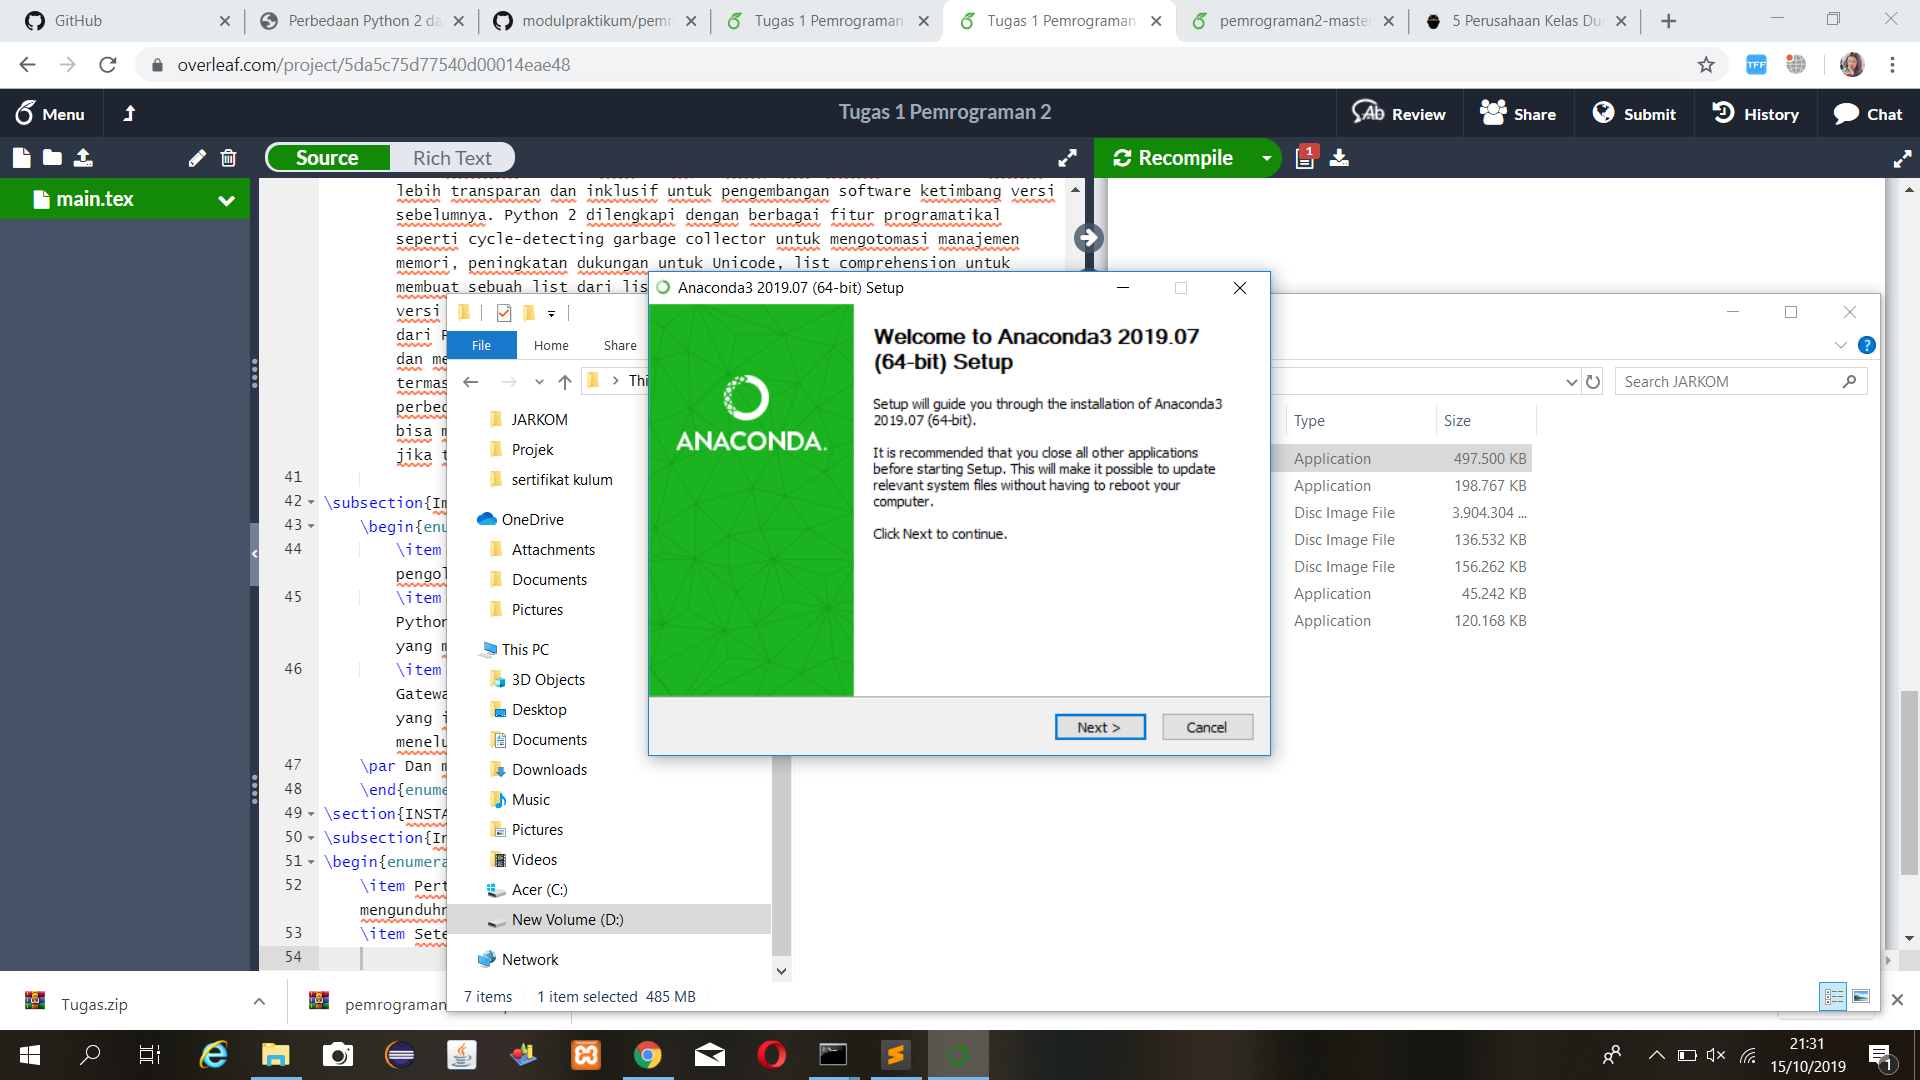
\includegraphics[width=8cm]{image/1.png}}
        \end{figure}
    \item Klik I agree, untuk menyetujui license instalasi Anaconda.
        \begin{figure}[h]
            \centerline{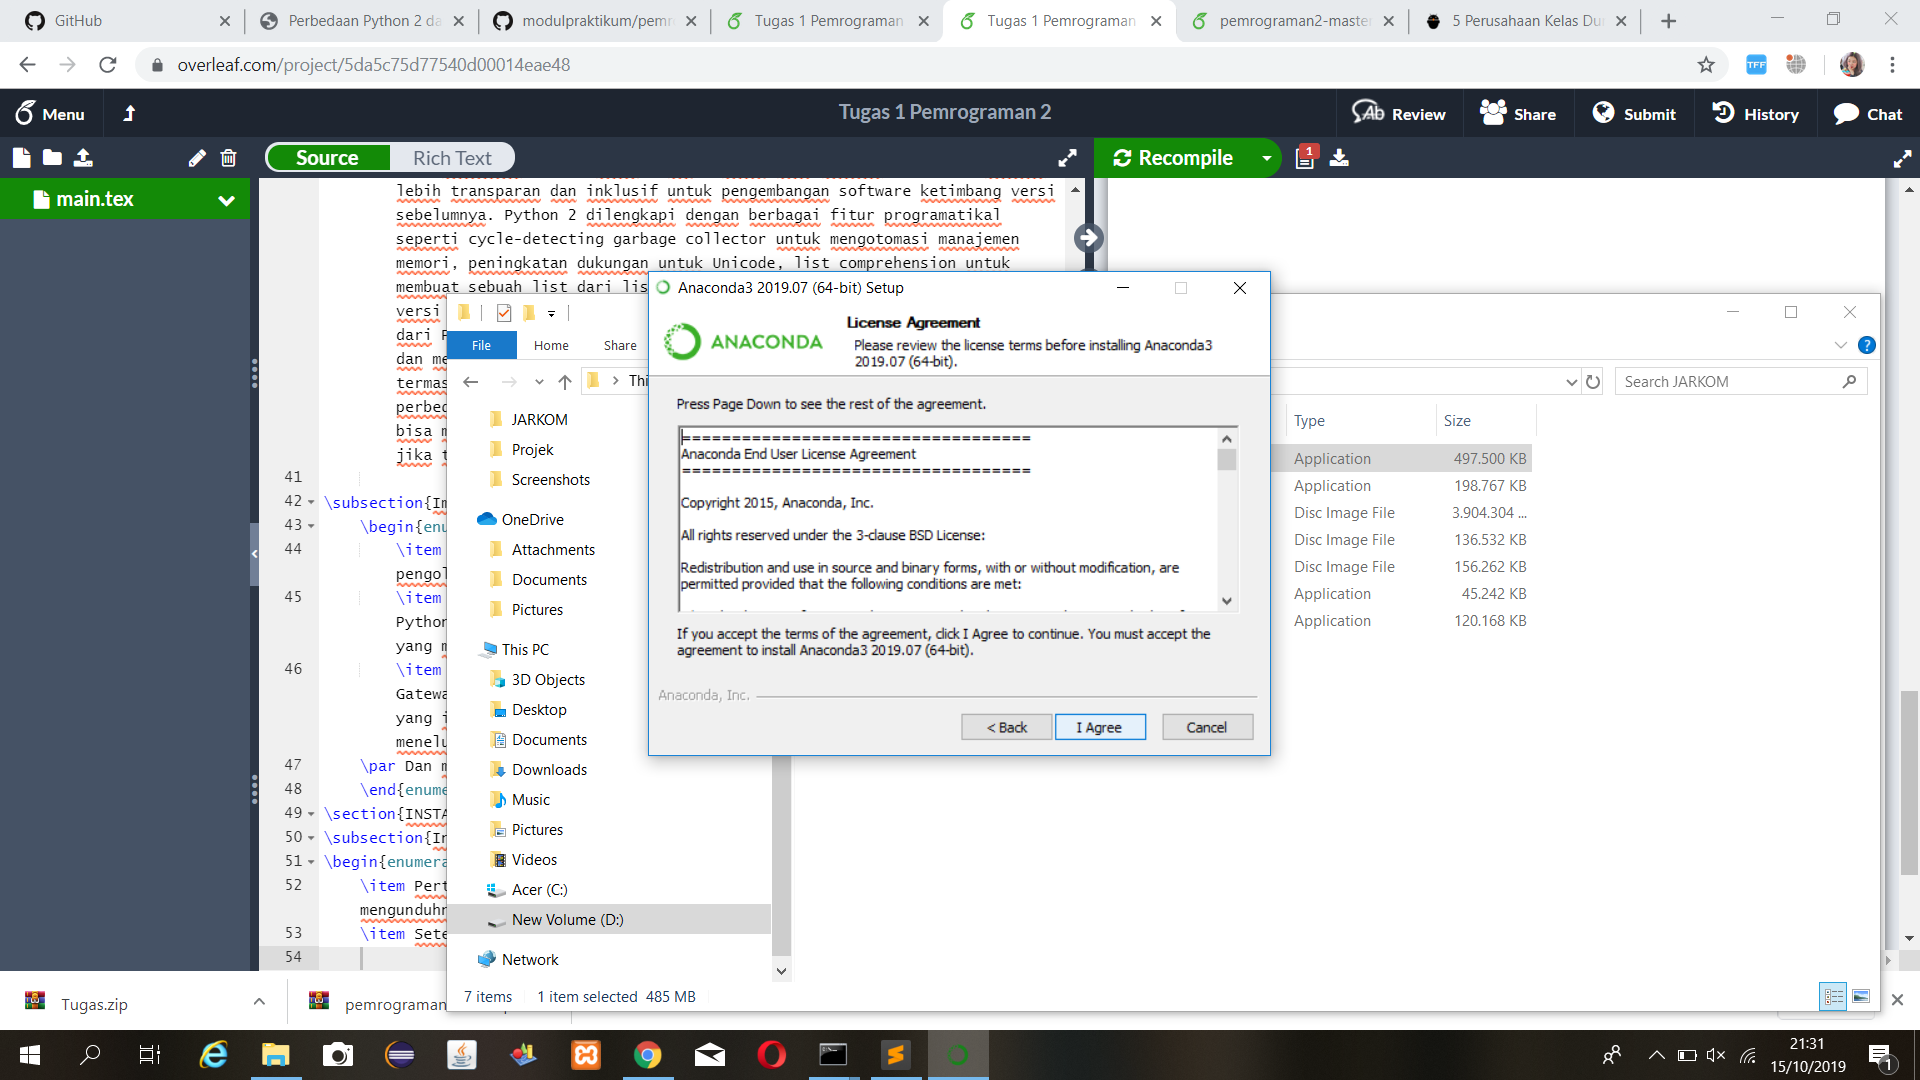
\includegraphics[width=8cm]{image/2.png}}
        \end{figure}
   \newpage
   \item Lalu pilih installation tipe, klik just me (yg direkomendasikan).
        \paragraph{}
            \centerline{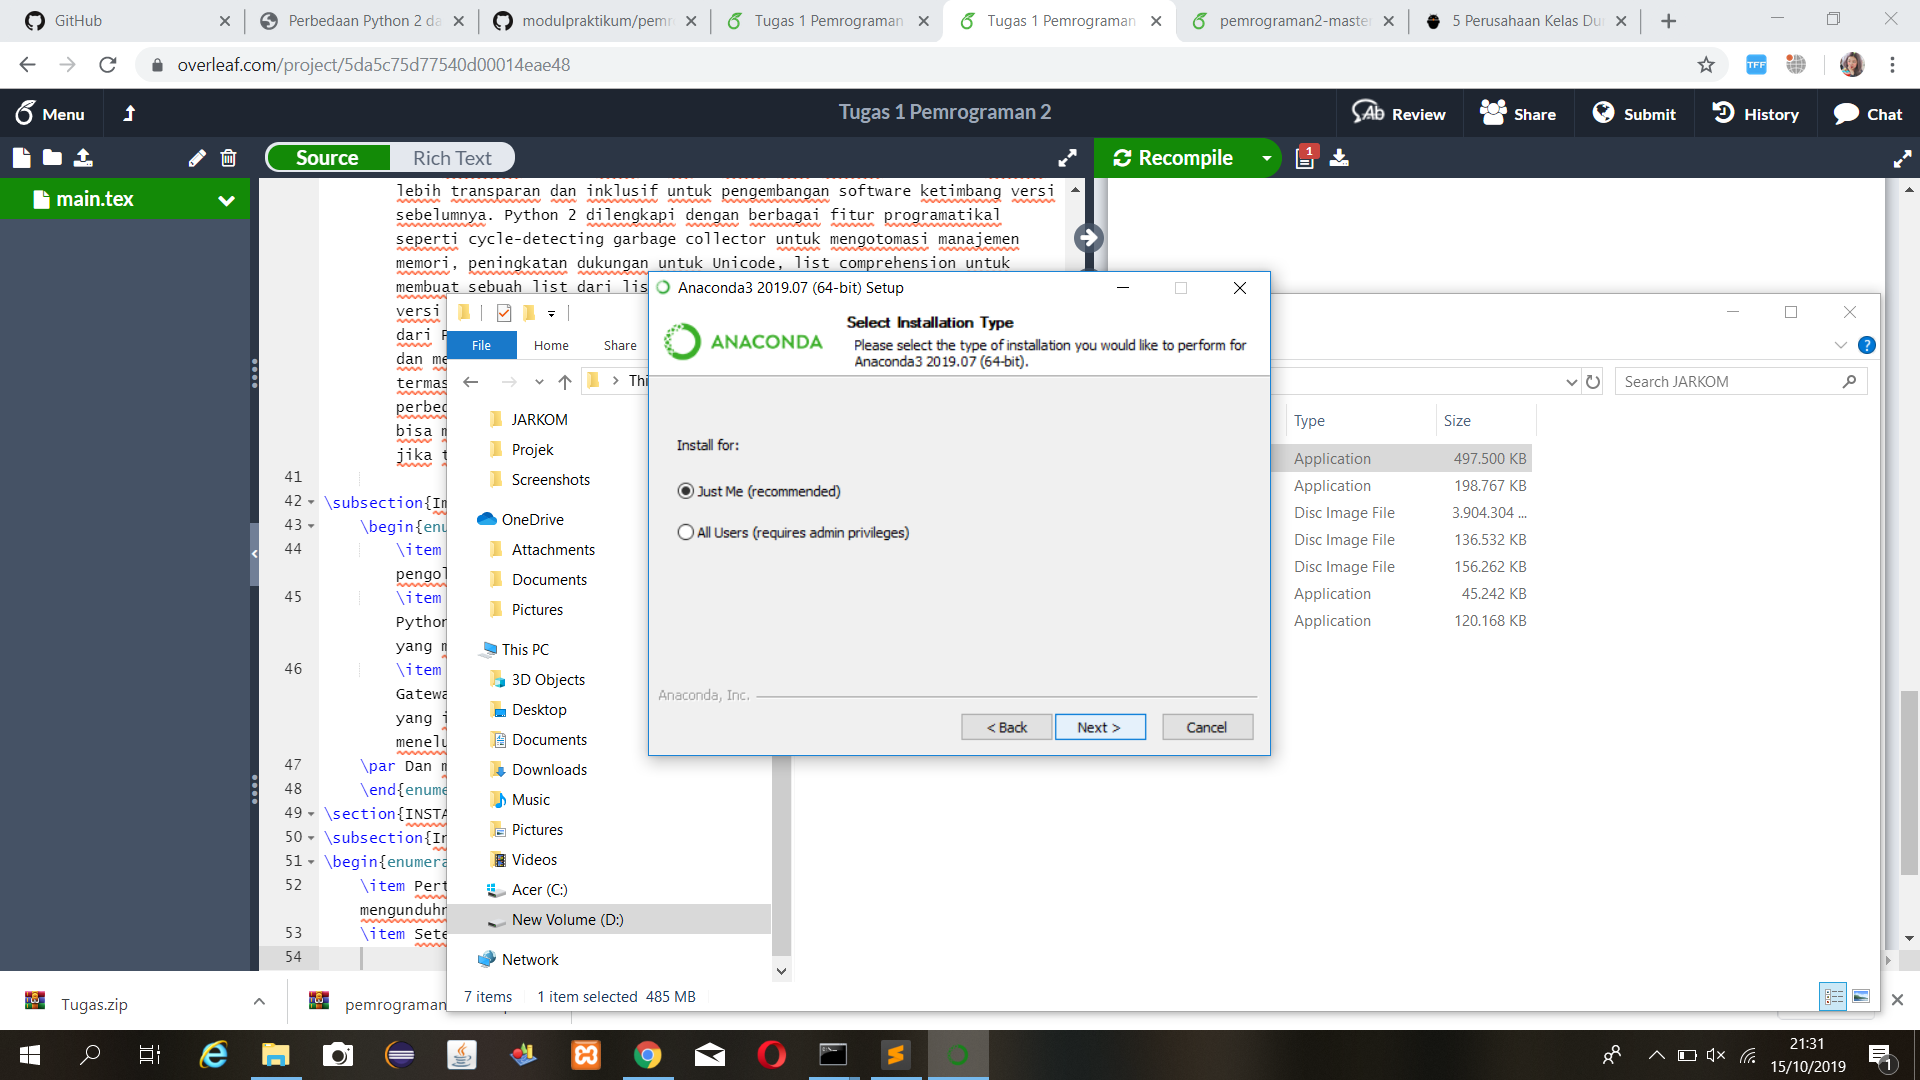
\includegraphics[width=8cm]{image/3.png}}
    \item Lalu pilih tempat atau lokasi direktori untuk instalasi Anaconda, klik next.
        \begin{figure}[h]
            \centerline{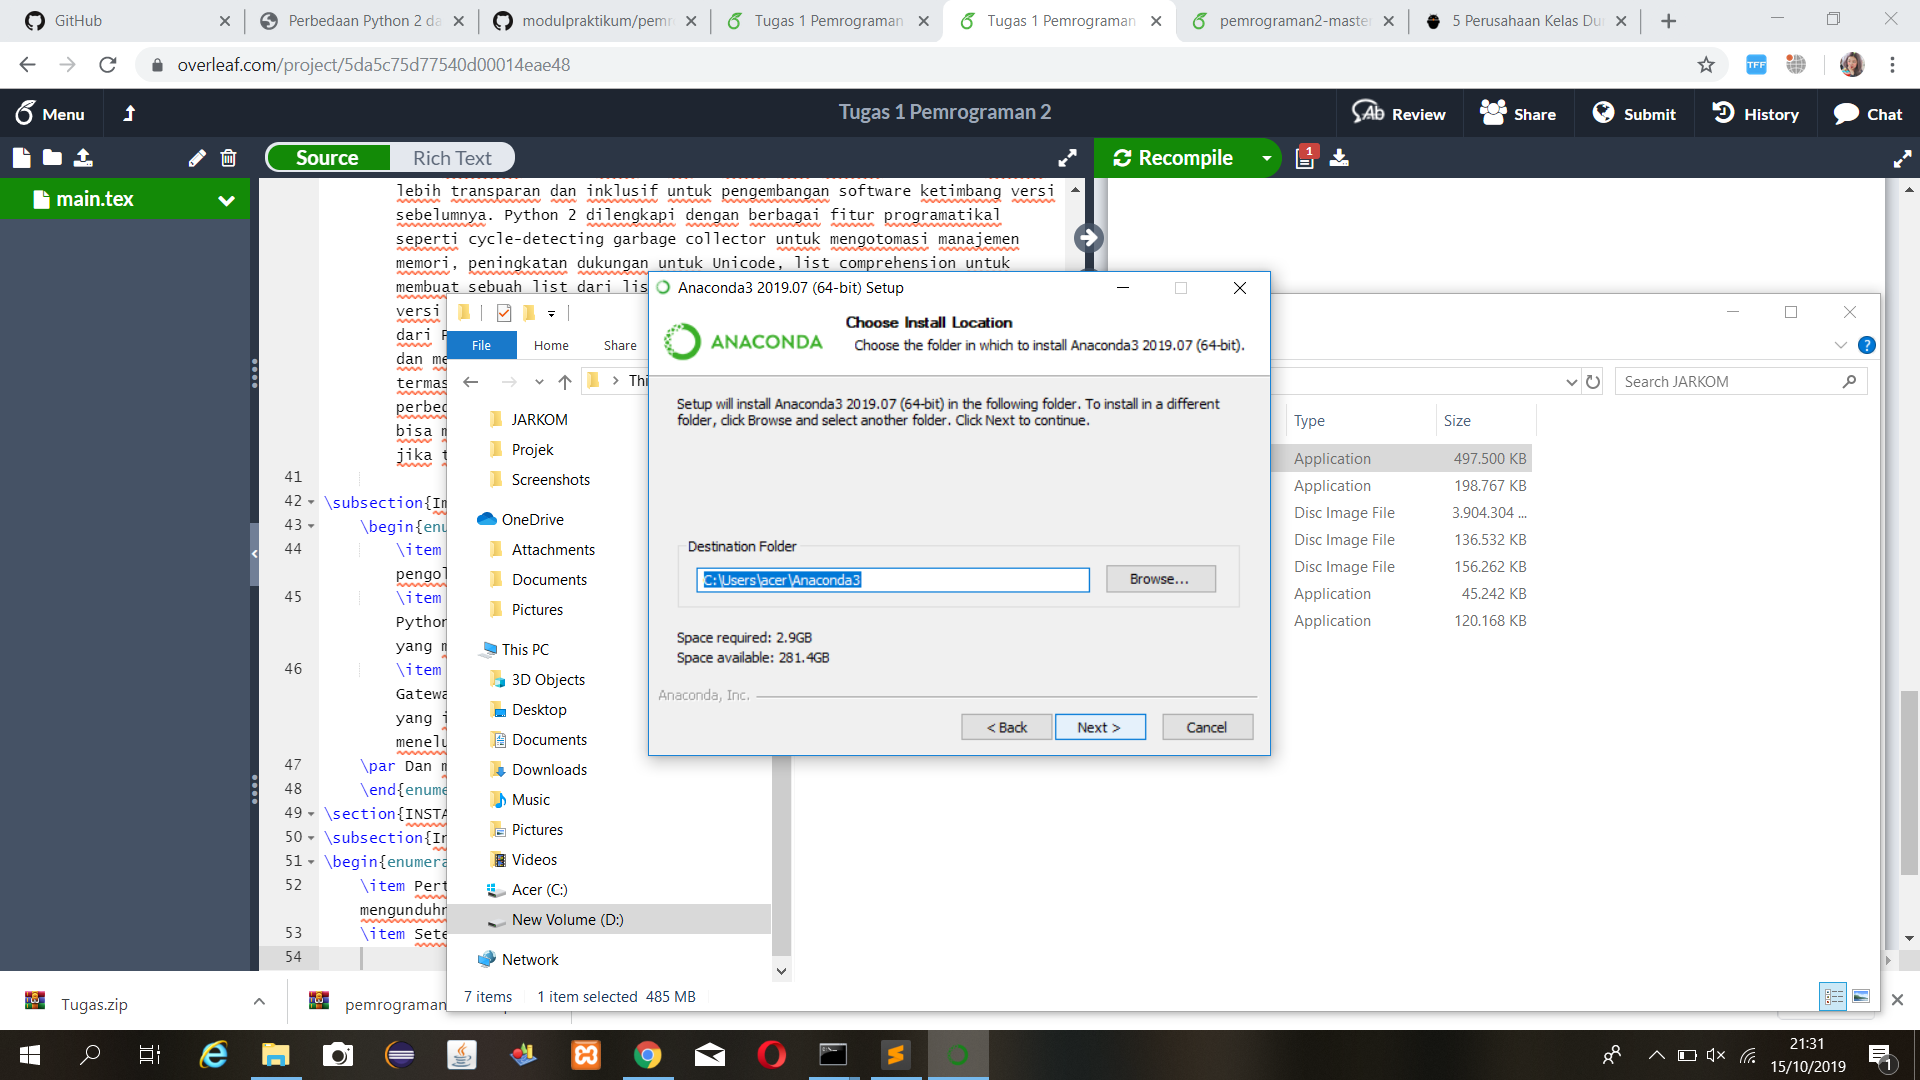
\includegraphics[width=8cm]{image/4.png}}
        \end{figure}
    \item Untuk advance option, pilih dua opsi tersebut. Tunggu hingga instalasi Anaconda selesai.
        \begin{figure}[h]
            \centerline{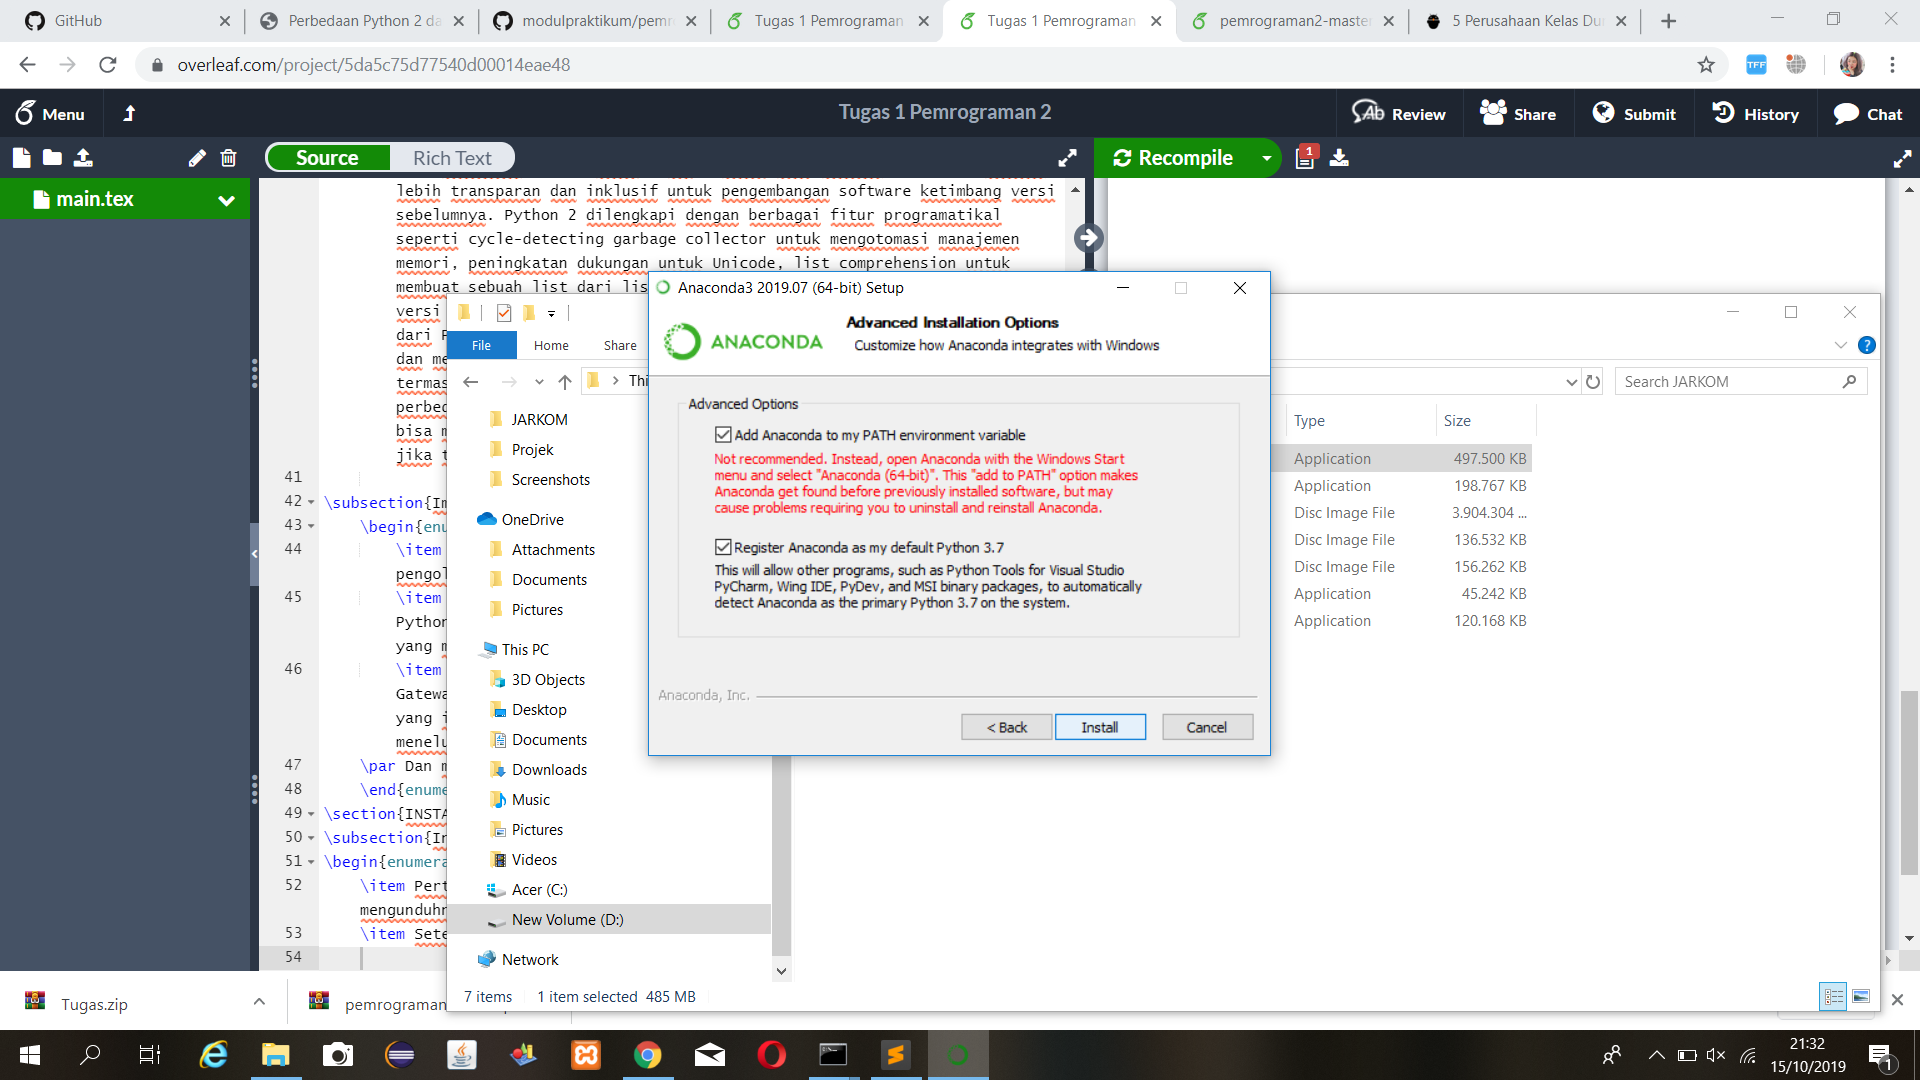
\includegraphics[width=8cm]{image/5.png}}
        \end{figure}
\end{enumerate}

\newpage
\subsection{Instalasi PIP}
\begin{enumerate}
    \item Pertama buka Anaconda promt atau dengan meng-klik tombol jendela windows dan huruf R secara bersamaan, maka akan menampilkan gambar seperti di bawah. Pilih cmd kemudian tekan OK.
        \begin{figure}[h]
            \centerline{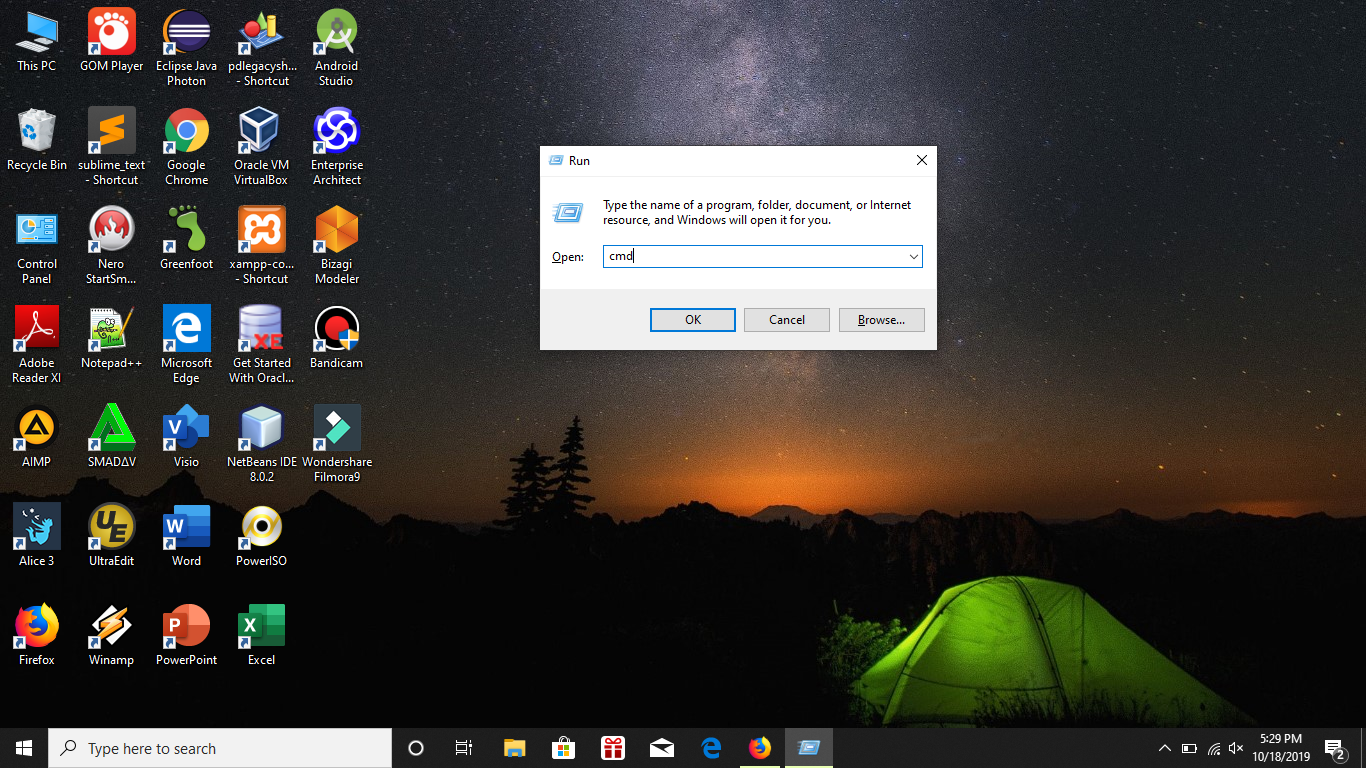
\includegraphics[width=8cm]{image/cmd.png}}
        \end{figure}
    \item Lalu ketikkan pip install requests.
        \begin{figure}[h]
            \centerline{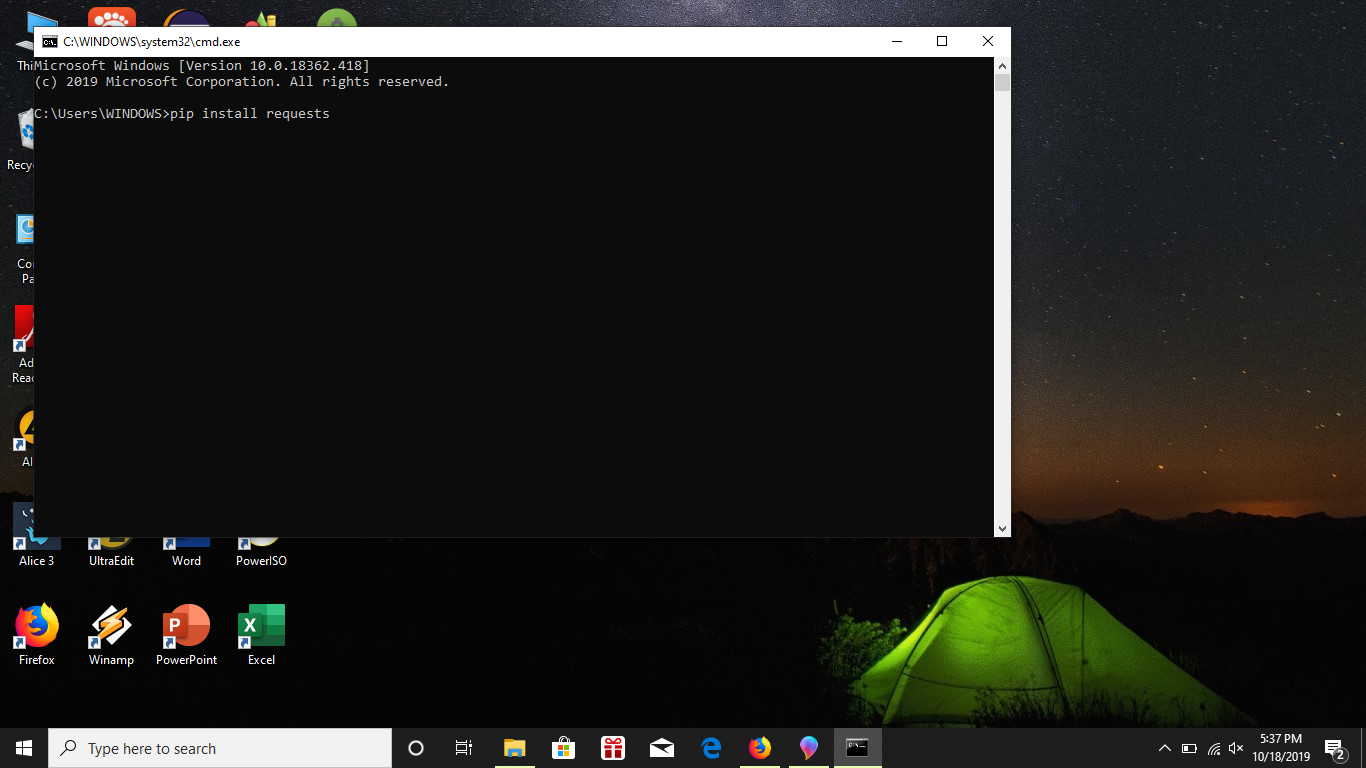
\includegraphics[width=8cm]{image/pip.png}}
        \end{figure}
    \item Jika berhasil maka akan keluar seperti berikut, jika gagal maka akan muncul pesan error.
            \paragraph{}
            \centerline{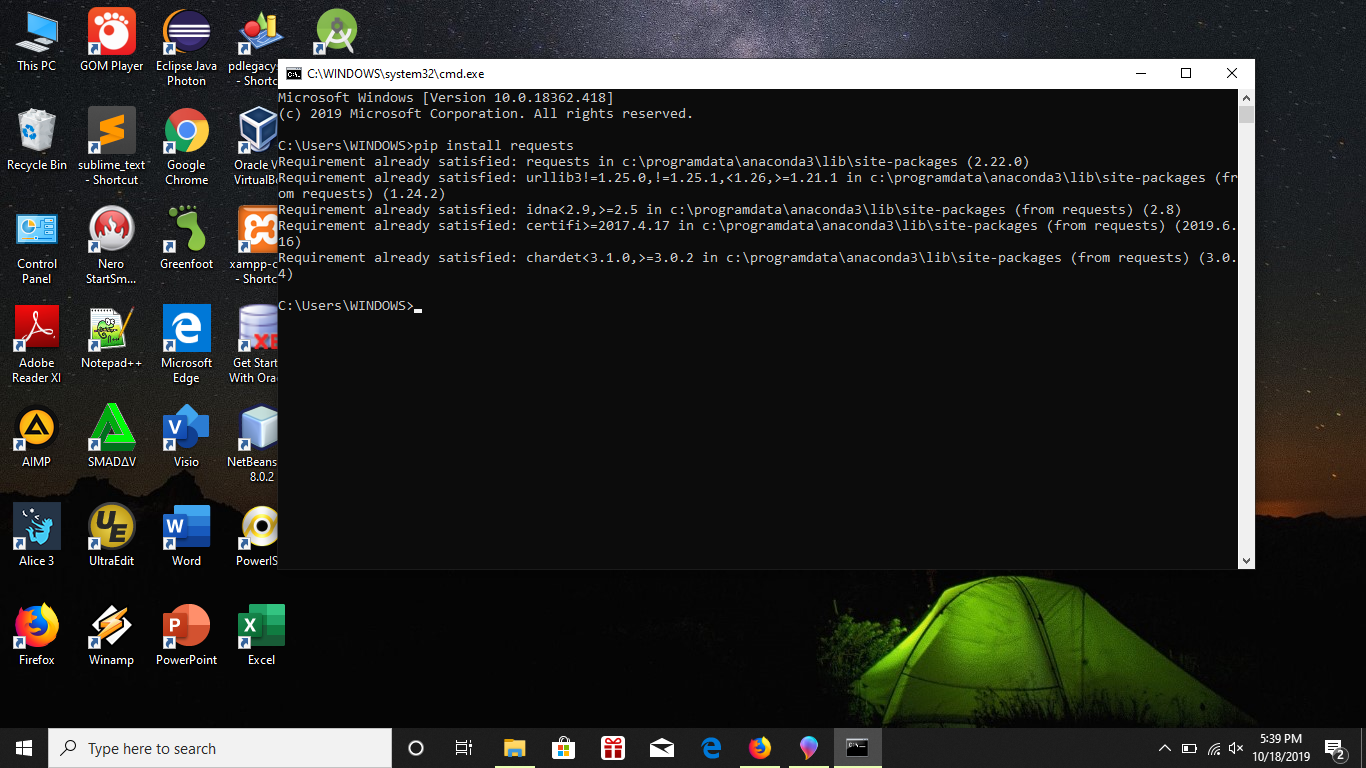
\includegraphics[width=8cm]{image/pipberhasil.png}}
\end{enumerate}

\subsection{Setting Environment}
\begin{enumerate}
    \item Pertama masuk ke control panel lalu pilih system dan security
        \begin{figure}[h]
            \centerline{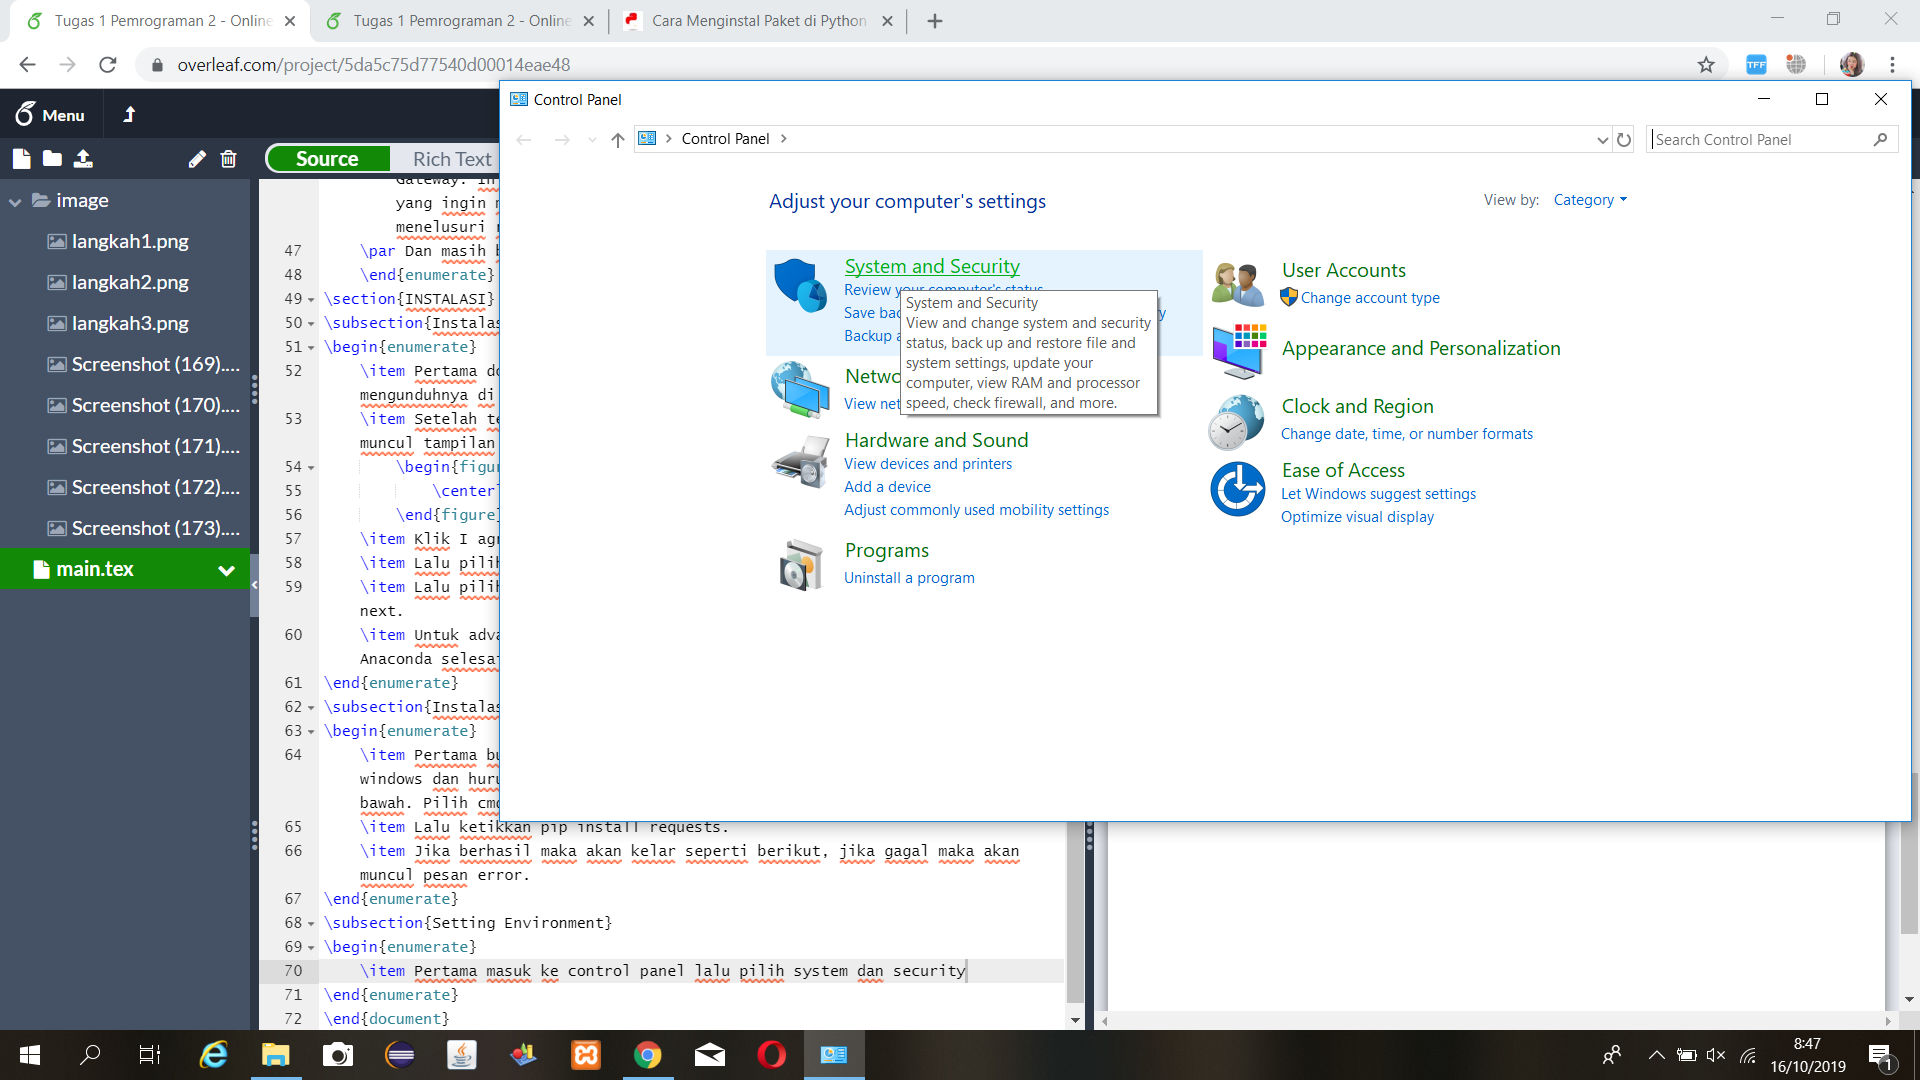
\includegraphics[width=8cm]{image/cpanel.png}}
        \end{figure}
    \item Lalu pilih Security and Maintanance
        \begin{figure}[h]
            \centerline{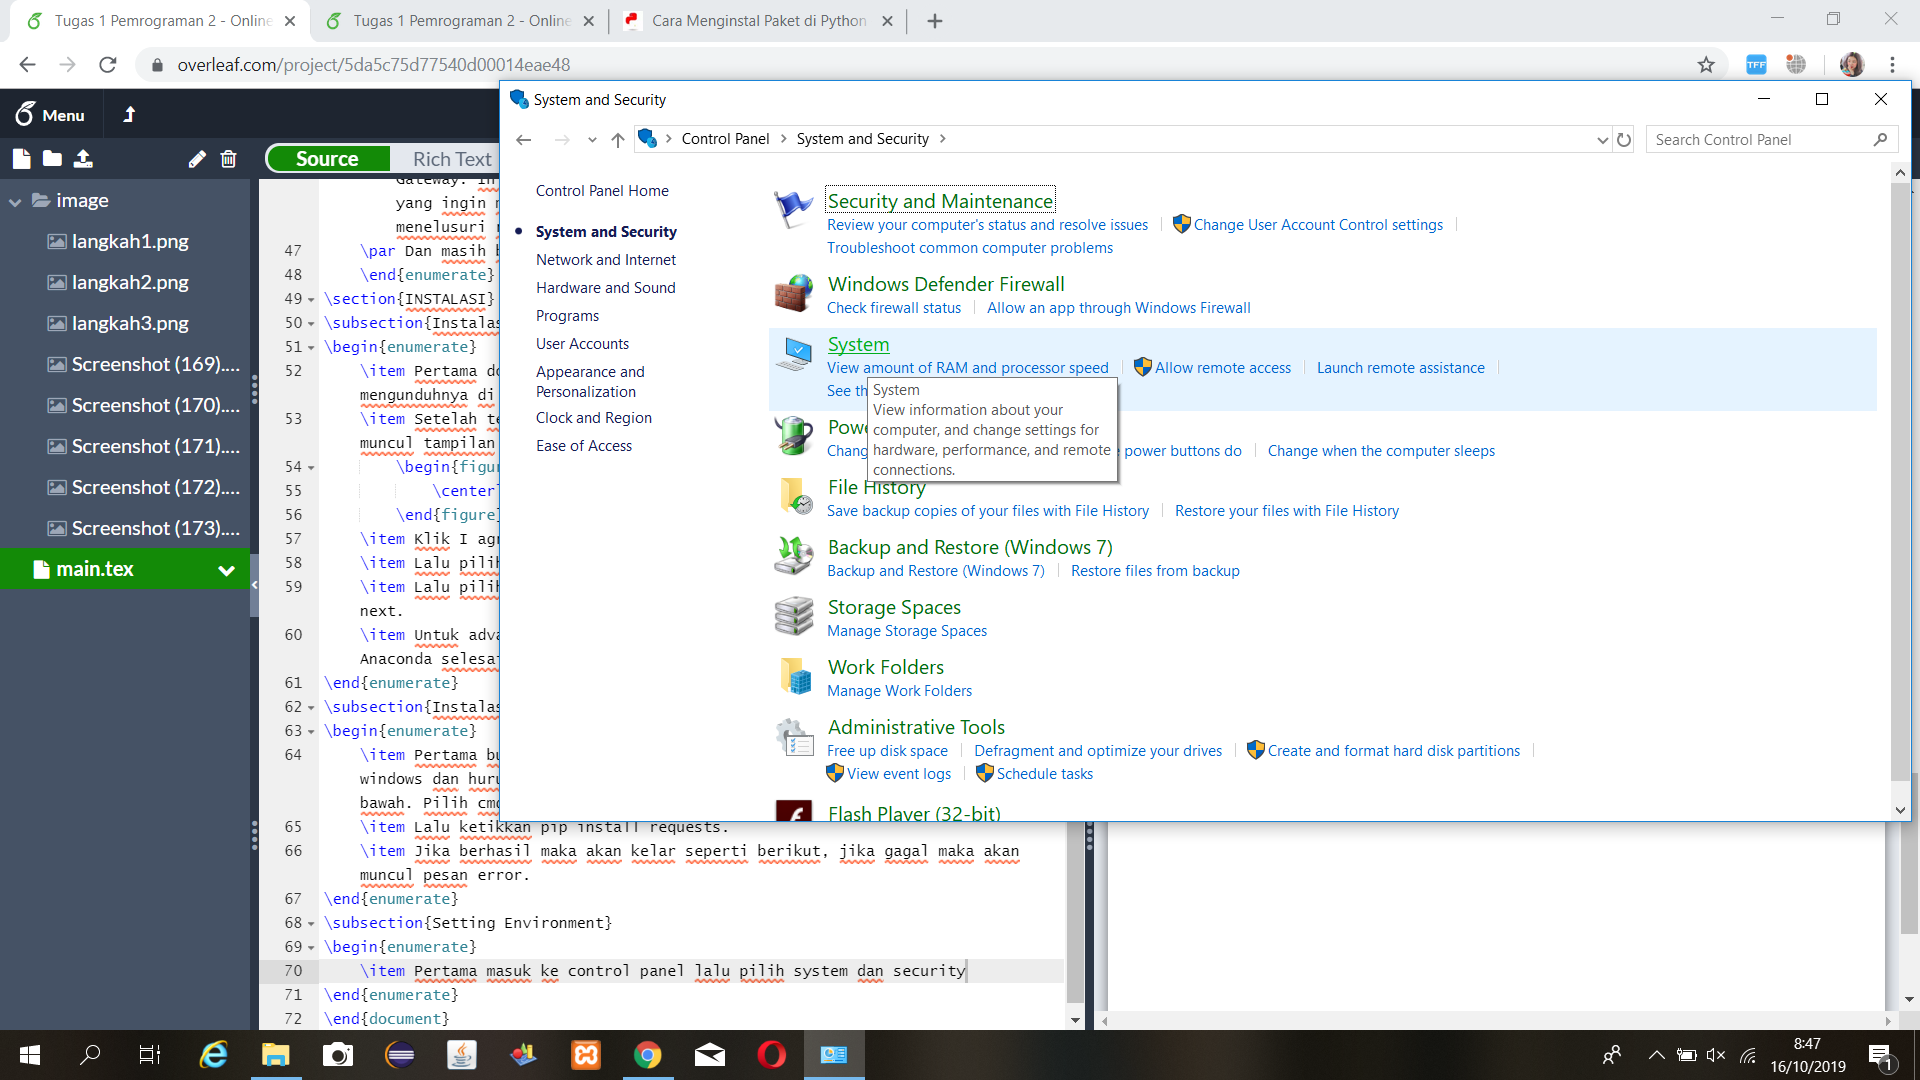
\includegraphics[width=8cm]{image/securityandmain.png}}
        \end{figure}
   \newpage
   \item Lalu pilih System dan Advanced System Settings.
            \paragraph{}
            \centerline{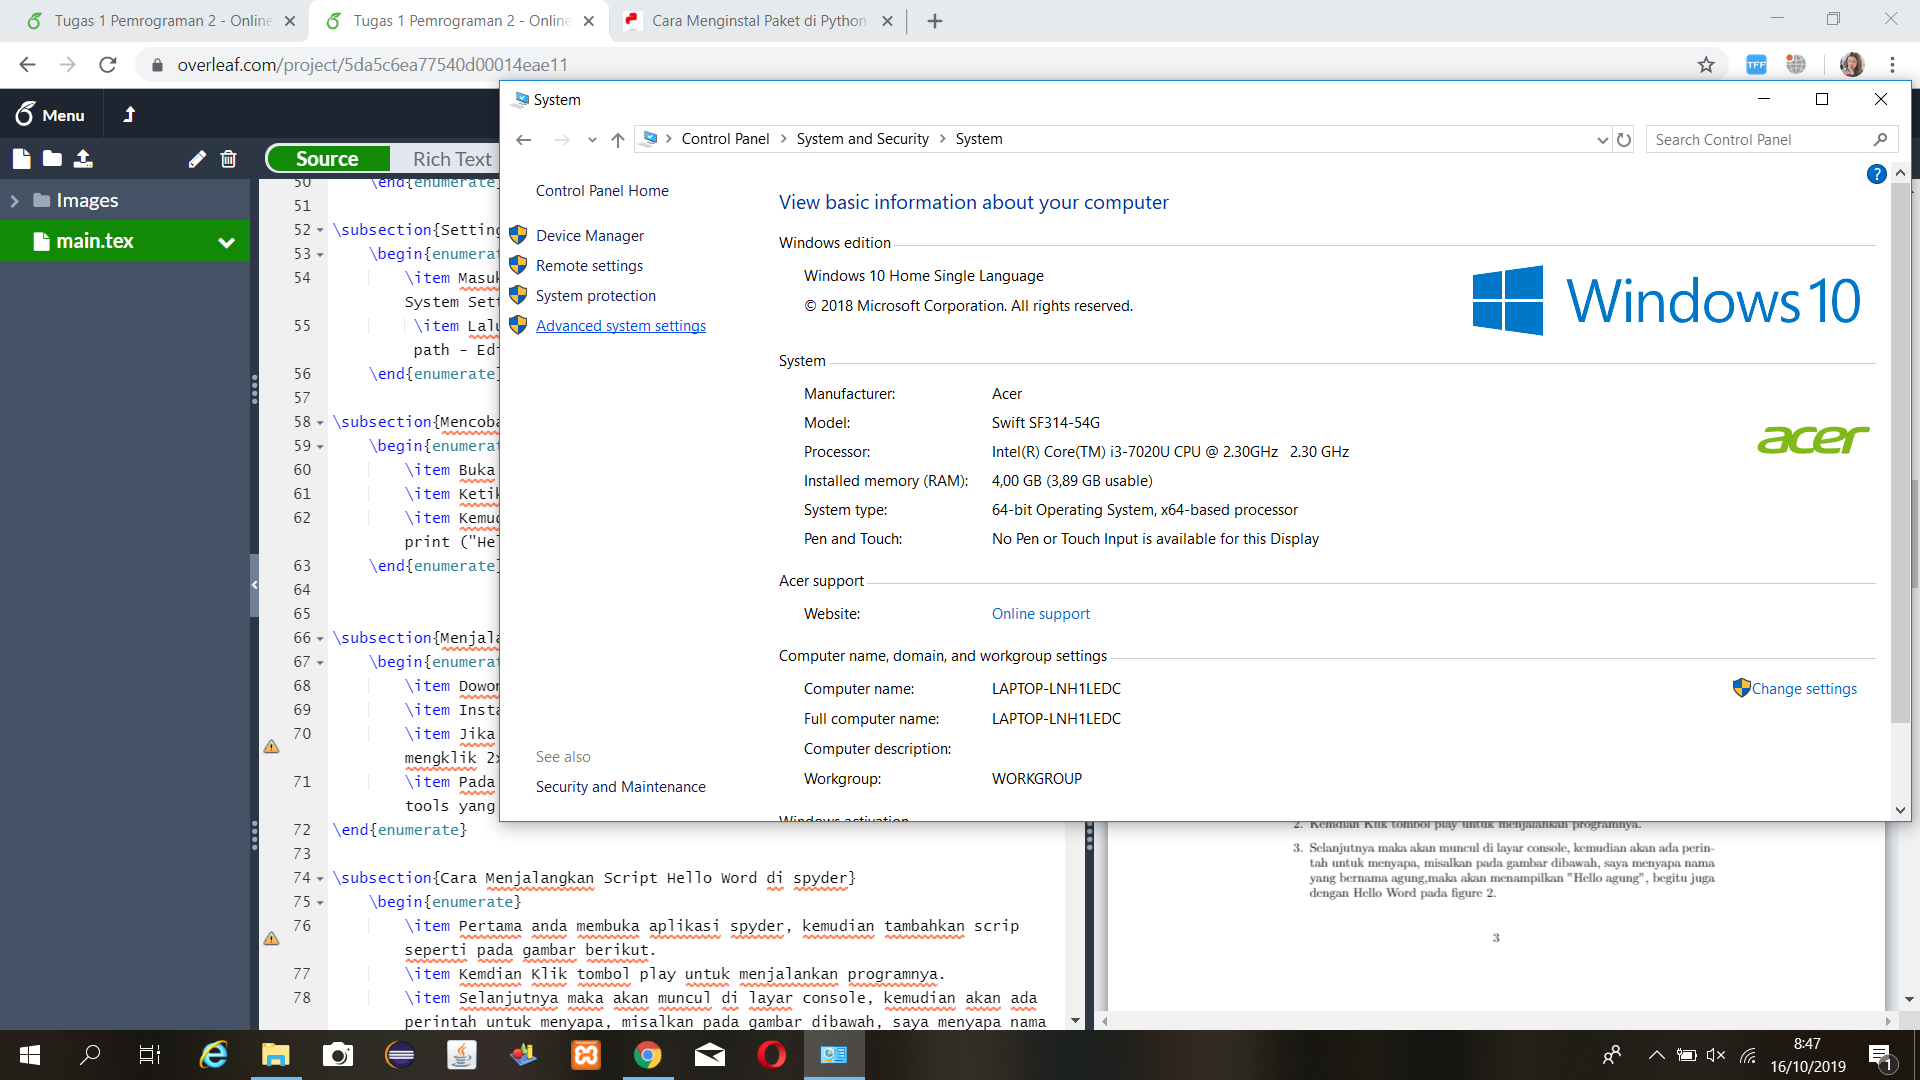
\includegraphics[width=8cm]{image/advanced.png}}
    \item Lalu pilih environment variables, lalu di System Variables klik path-Edit-New-C:/Python3/Scripts lalu klik OK.
        \begin{figure}[h]
            \centerline{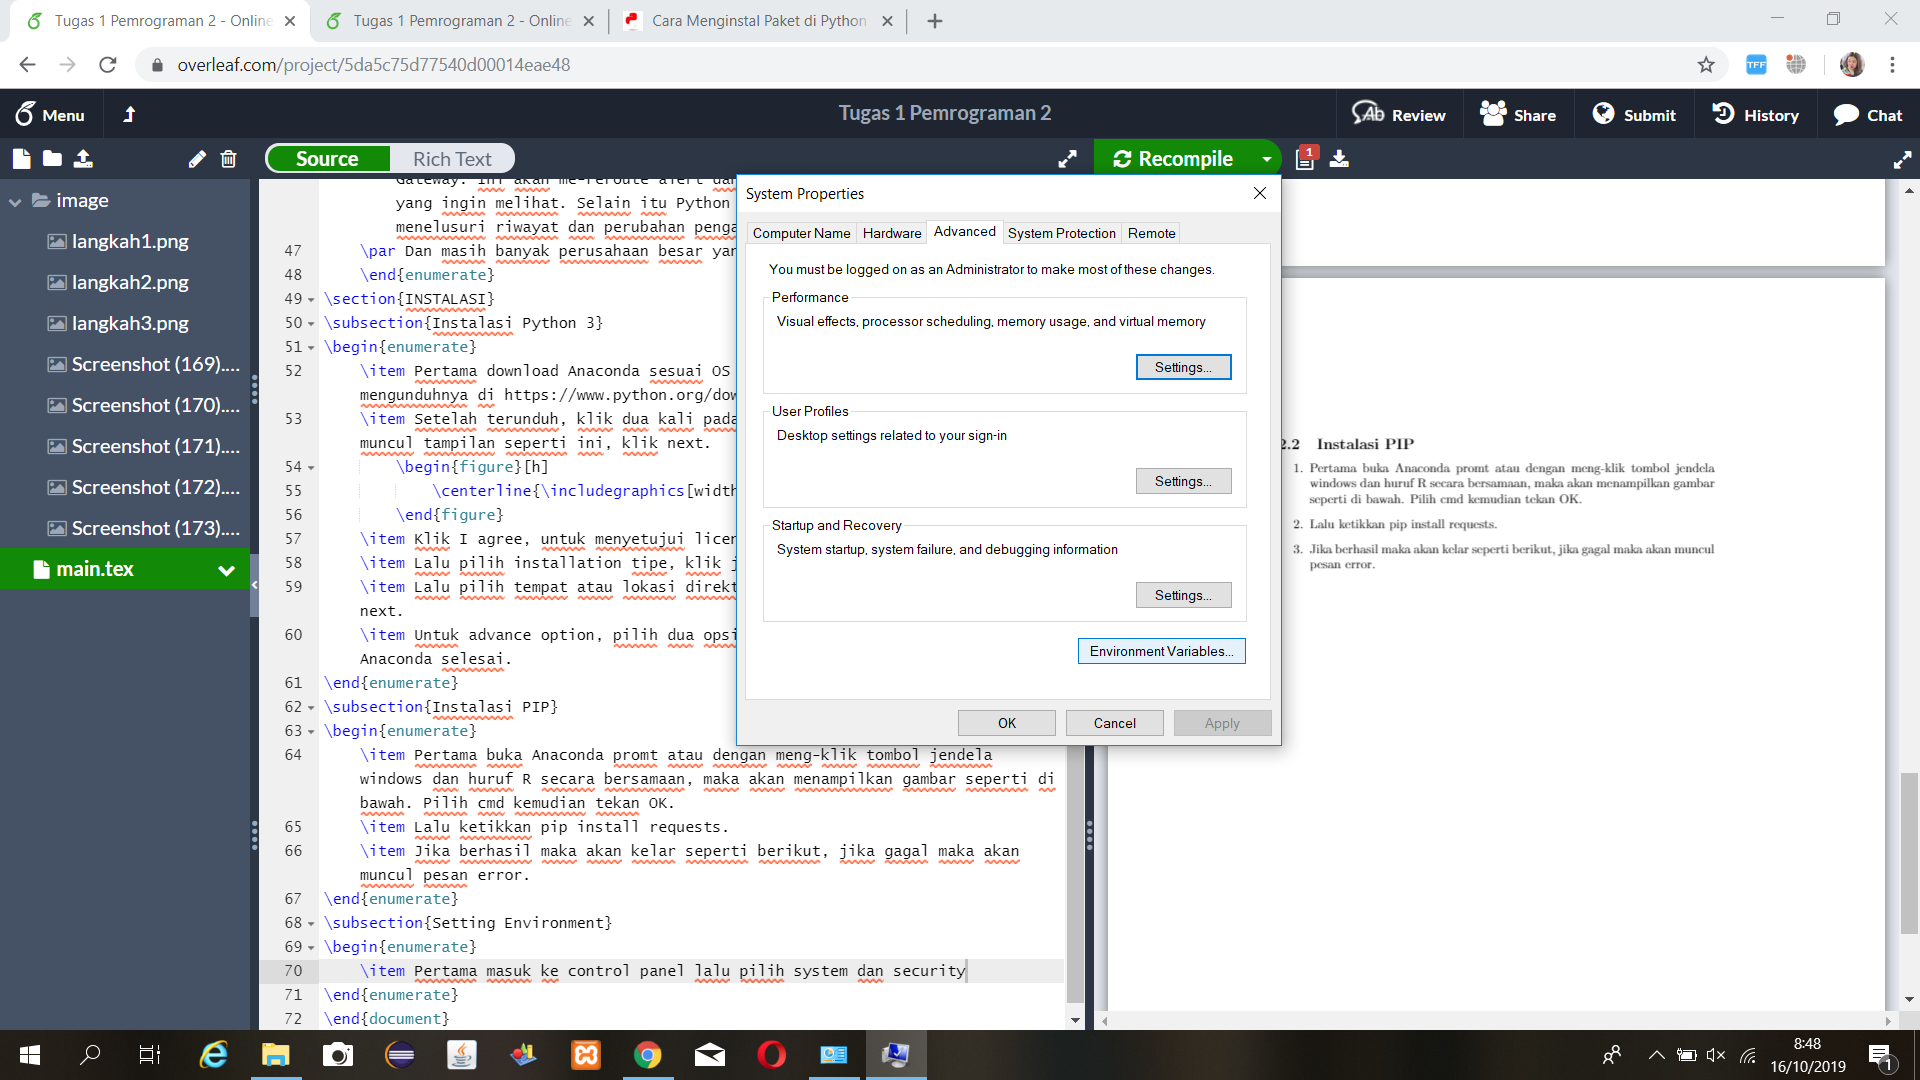
\includegraphics[width=8cm]{image/environtmentvar.png}}
        \end{figure}
        \begin{figure}[h]
            \centerline{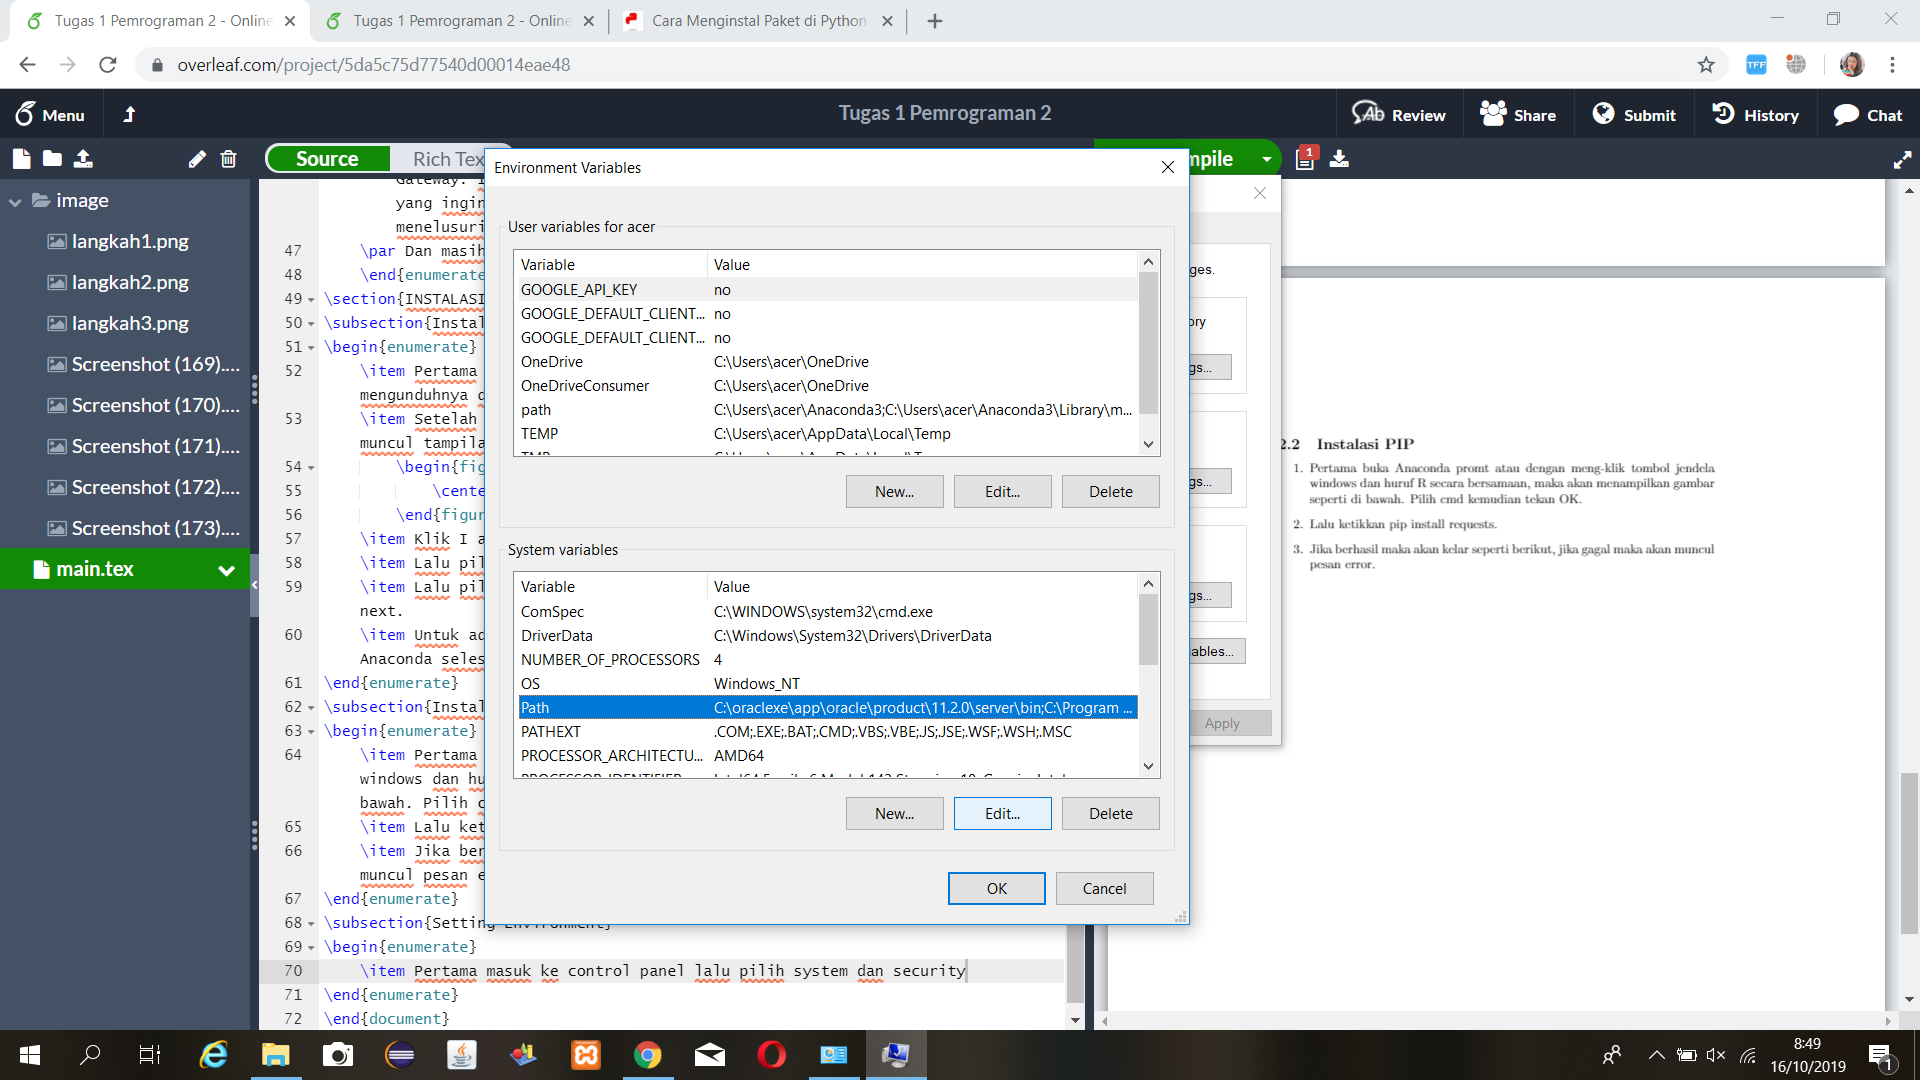
\includegraphics[width=8cm]{image/pathedit.png}}
        \end{figure}
        \paragraph{}
            \centerline{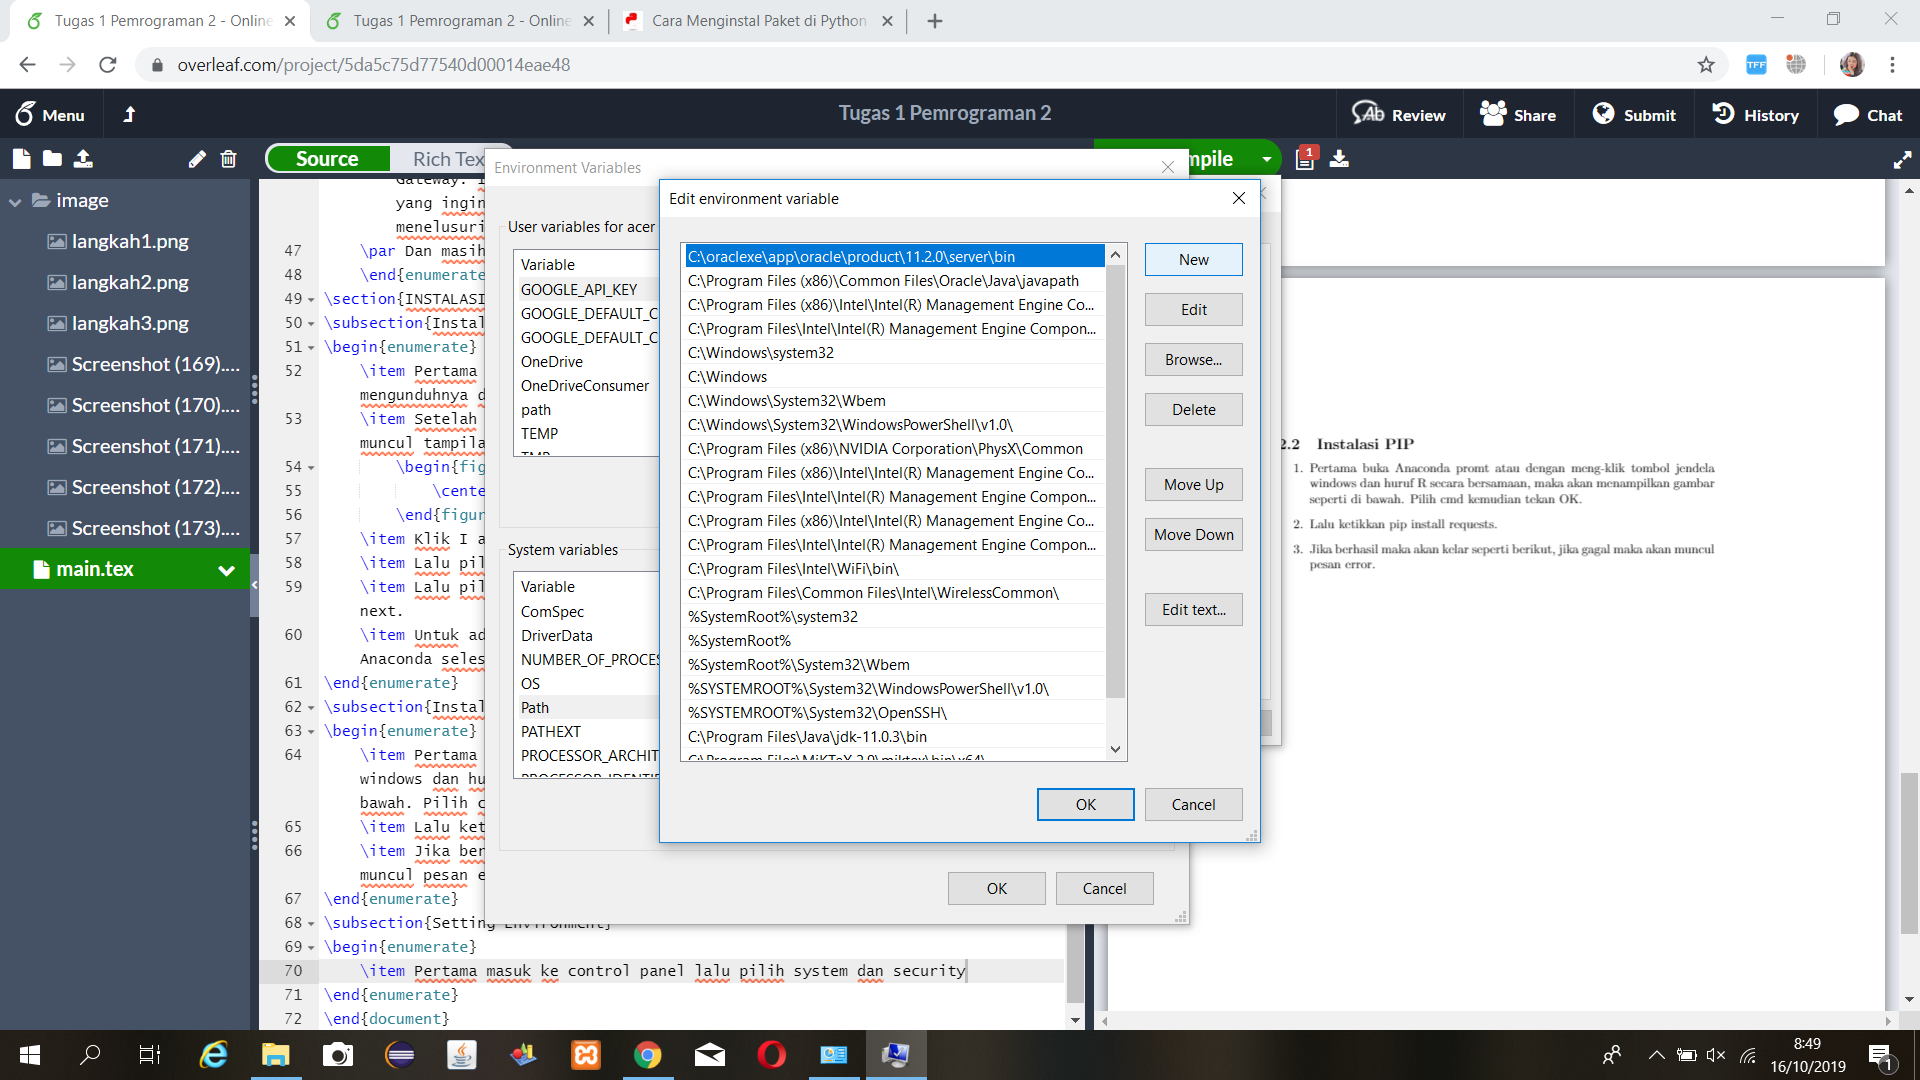
\includegraphics[width=8cm]{image/new.png}}
        \paragraph{}
            \centerline{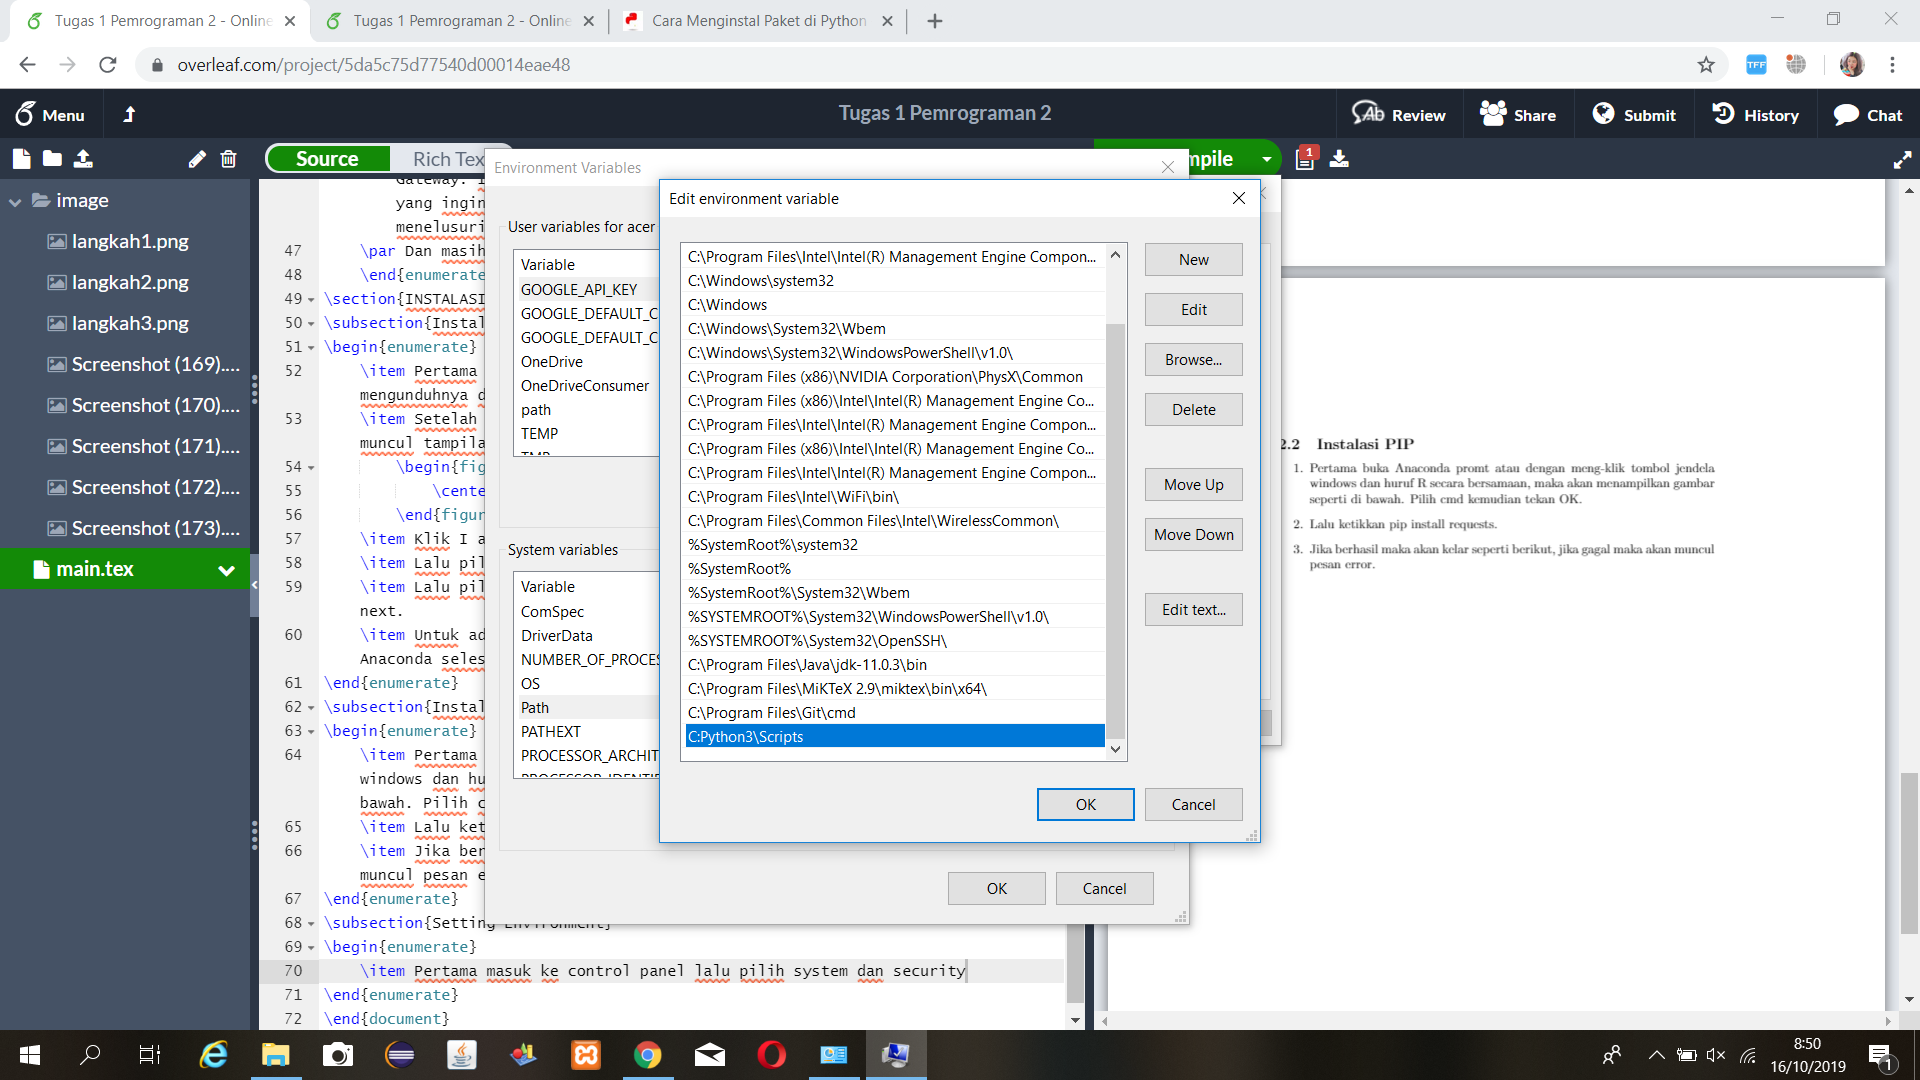
\includegraphics[width=8cm]{image/pathnewok.png}}
\end{enumerate}
\subsection{Mencoba Interpreter/CLI pada CMD}
\begin{enumerate}
    \item Pertama buka Cmd terlebih dahulu pada PC/Laptop anda.
        \begin{figure}[h]
            \centerline{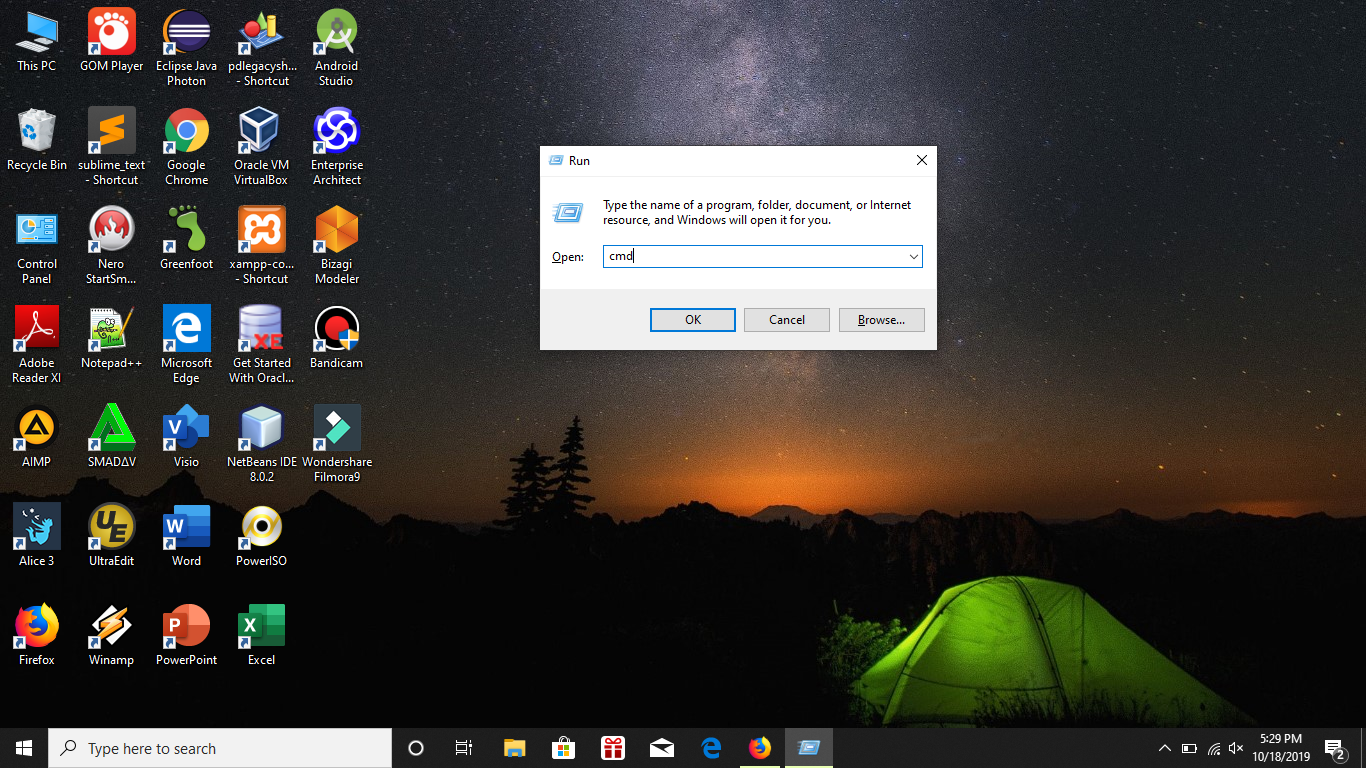
\includegraphics[width=8cm]{image/cmd.png}}
        \end{figure}
    \item Kemudian ketikkan Python
        \begin{figure}[h]
            \centerline{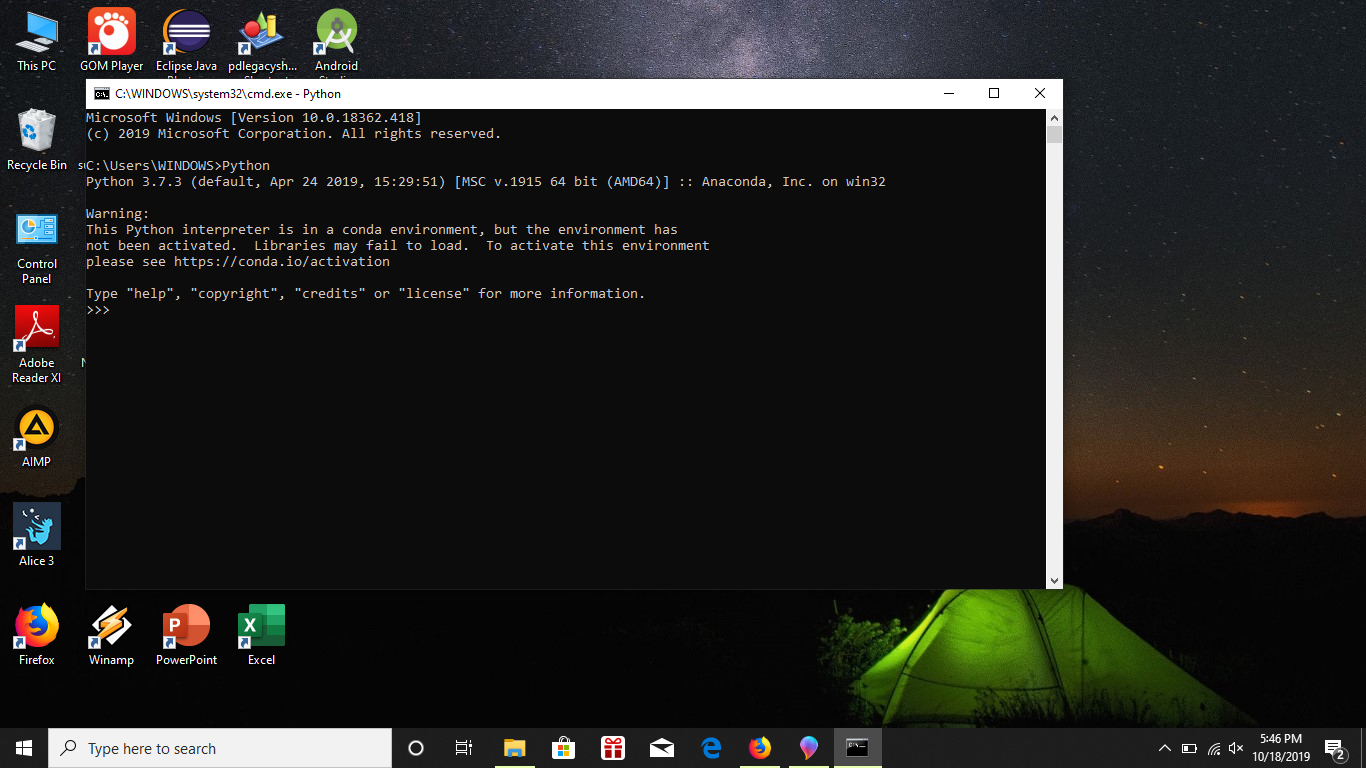
\includegraphics[width=8cm]{image/python.png}}
        \end{figure}
    \item Lalu ketikkan print("Hello World!")
    \paragraph{}
            \centerline{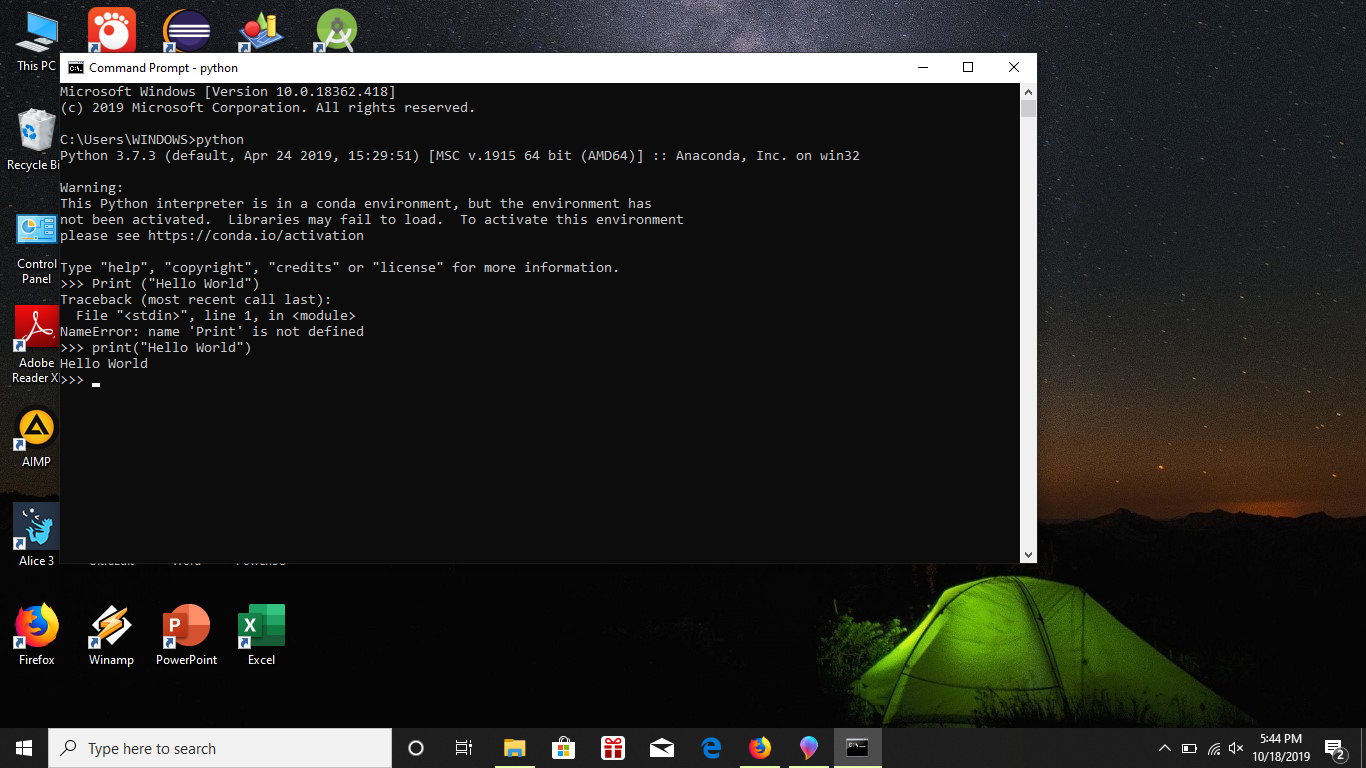
\includegraphics[width=8cm]{image/printhelloworld.png}}
\end{enumerate}
\subsection{Menjalankan dan Mengupdate Anaconda dan Spyder}
\begin{enumerate}
    \item Pertama download terlebih dahulu aplikasi Anaconda
    \item Lalu install
    \item Setelah terinstall buka Anaconda
    \item Di dalamnya terdapat Spyder dan lain lain.
    \item Untuk mengupdate Anaconda, silahkan pergi ke cmd lalu ketikkan Conda install -c anaconda python
        \begin{figure}[h]
            \centerline{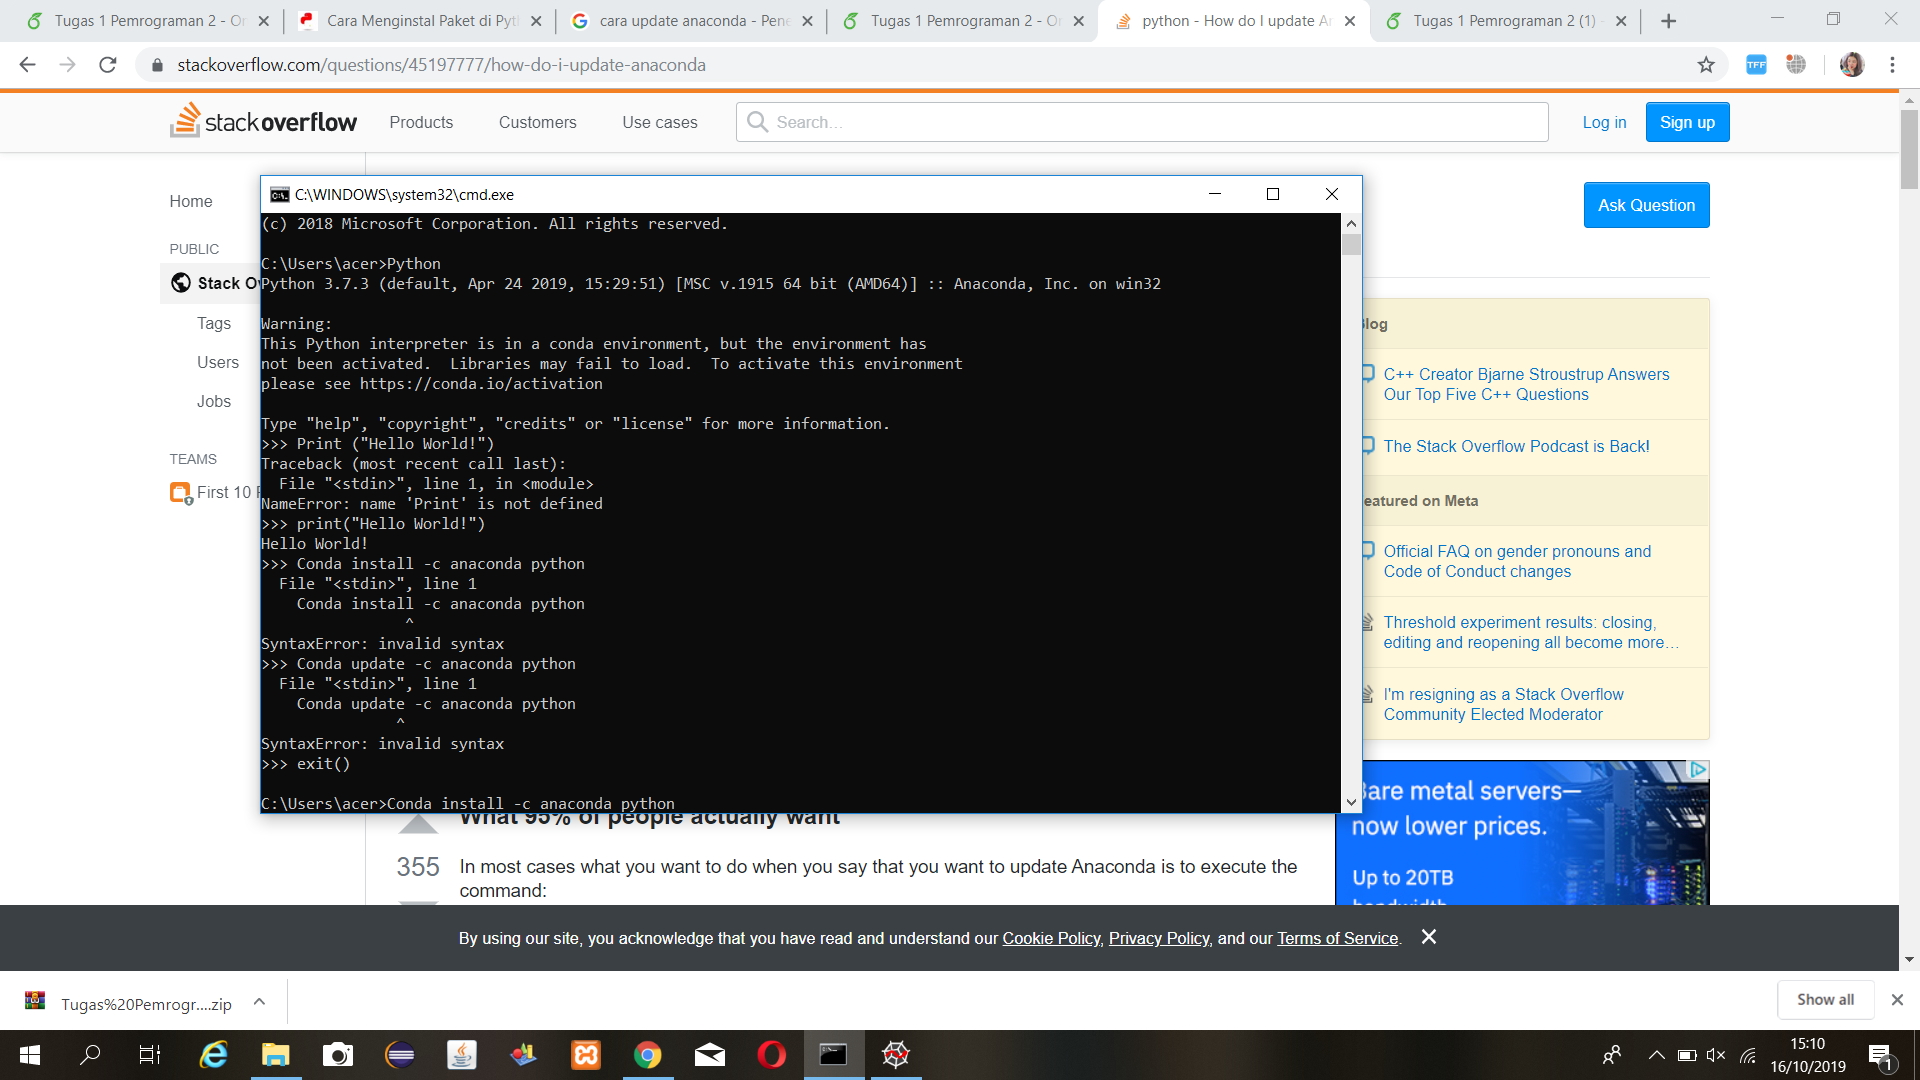
\includegraphics[width=8cm]{image/anacondaupdt.png}}
        \end{figure}
\end{enumerate}
\newpage
\subsection{Menjalankan Script "Hello World!" di Spyder}
\begin{enumerate}
    \item Pertama buka lah aplikasi Spyder
    \paragraph{}
            \centerline{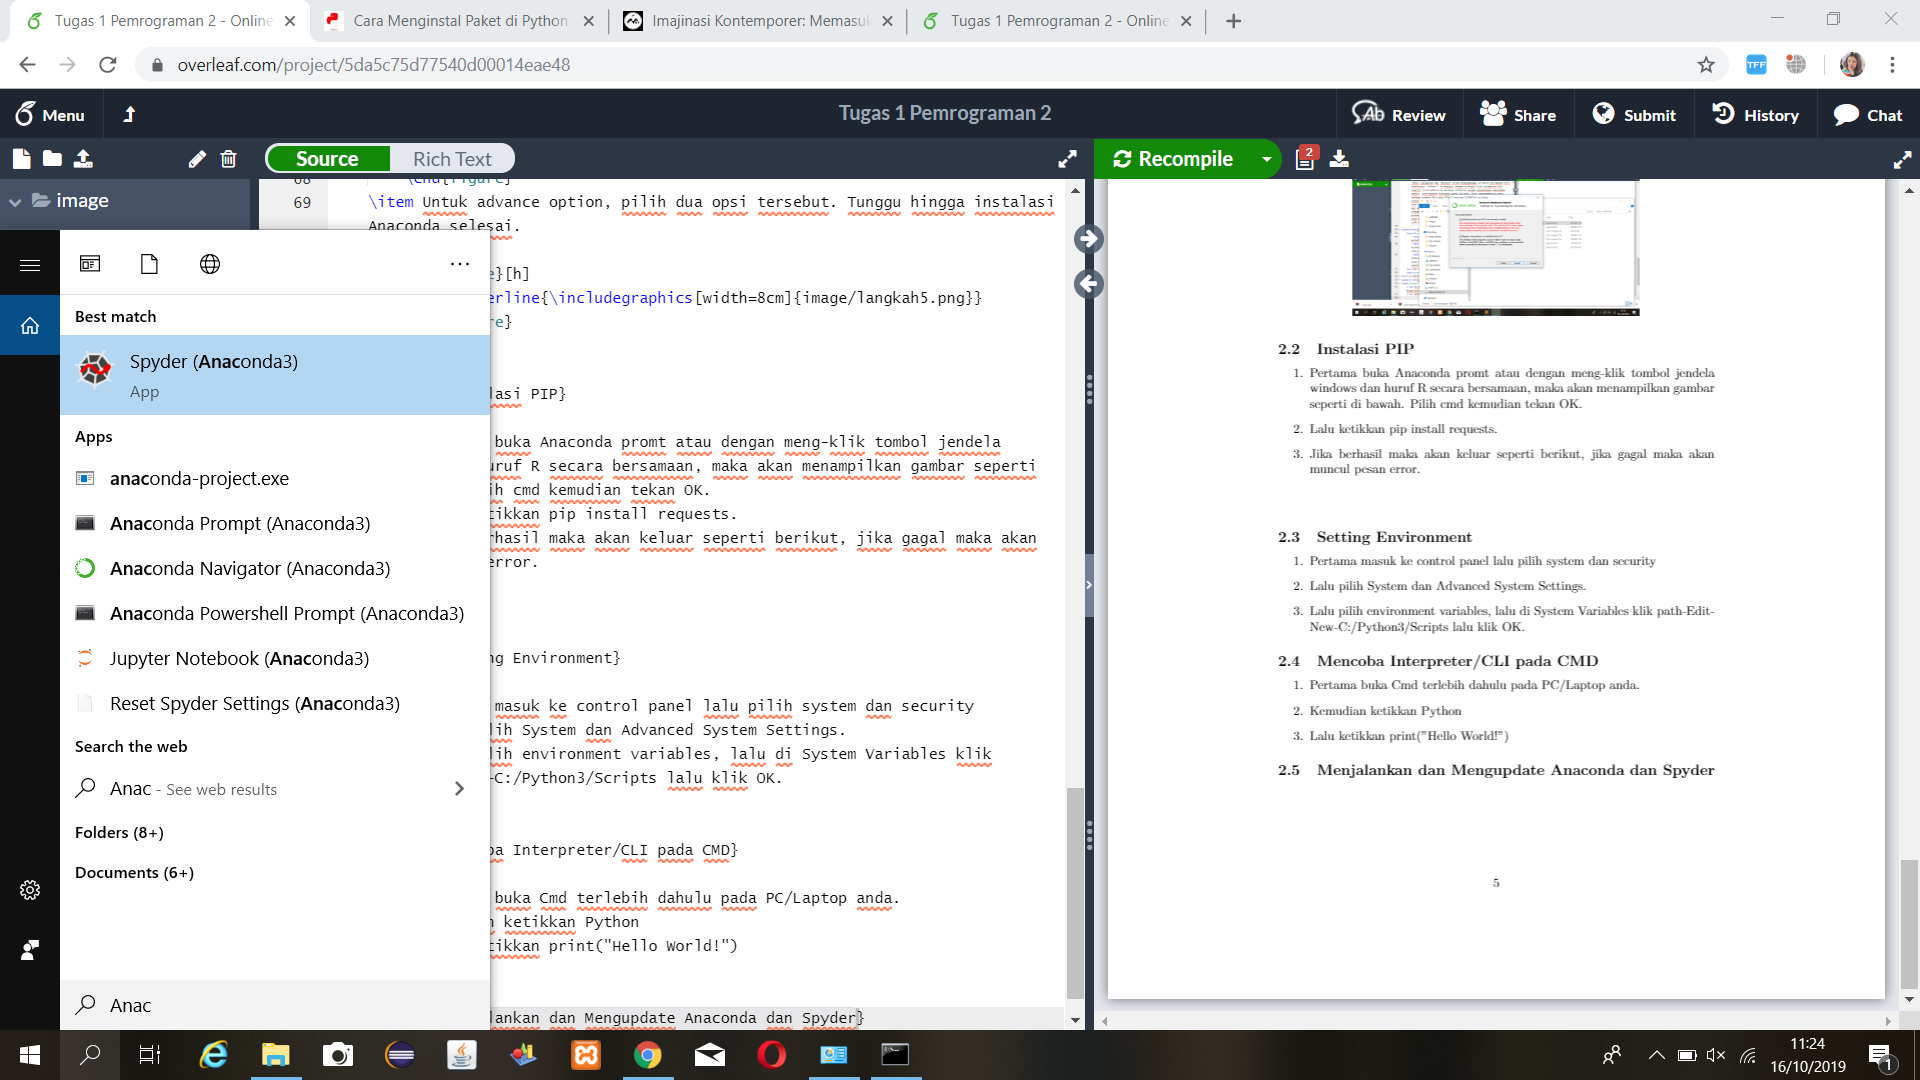
\includegraphics[width=8cm]{image/spyder.png}}
    \item Lalu ketikkan script seperti berikut
        \begin{figure}[h]
            \centerline{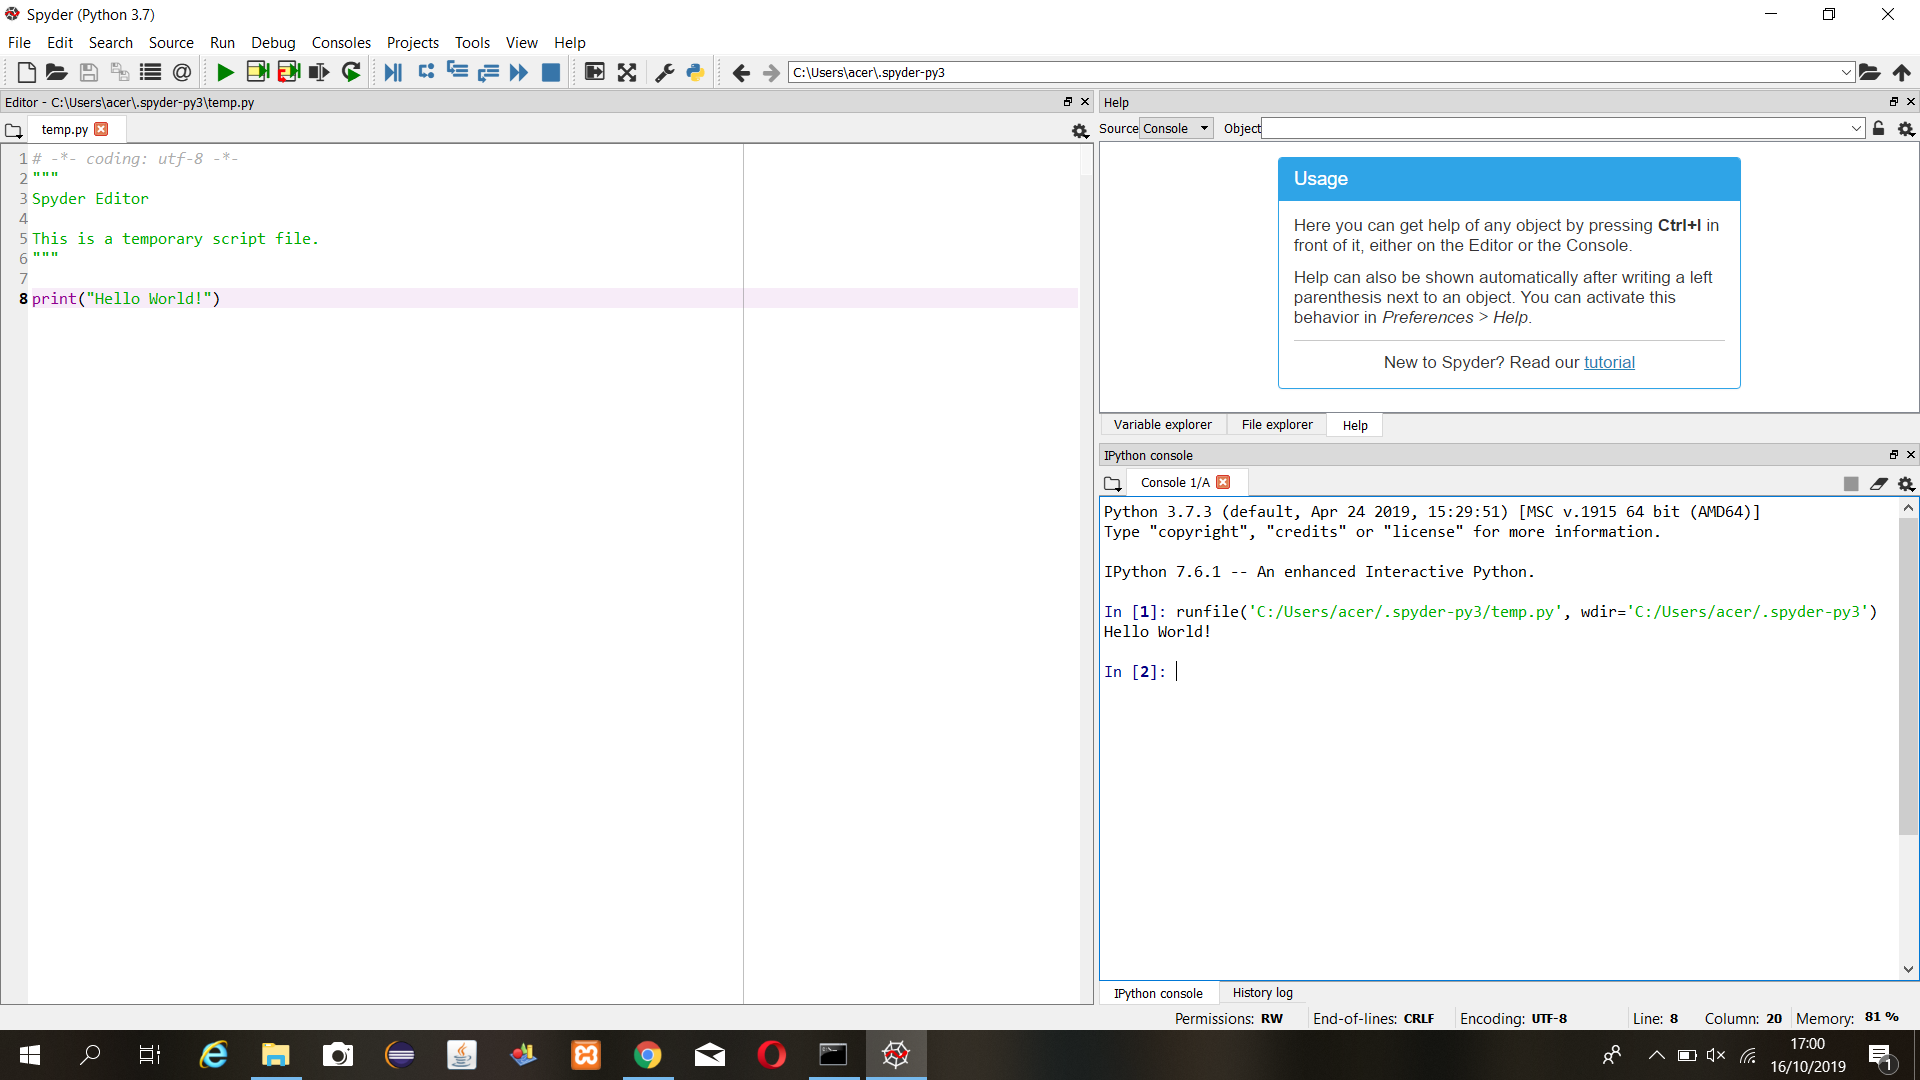
\includegraphics[width=8cm]{image/helloworld.png}}
        \end{figure}
    \item Lalu akan ditampilkan pada console, maka hasilnya "Hello World!"
\end{enumerate}

\subsection{Menjalankan Login Otomatis dengan Library Selenium dan Inputan User}
\begin{enumerate}
    \item Pertama buka cmd terlebih dahulu
    \item Lalu install Selenium dengan cara ketikkan "pip install selenium"
        \paragraph{}
            \centerline{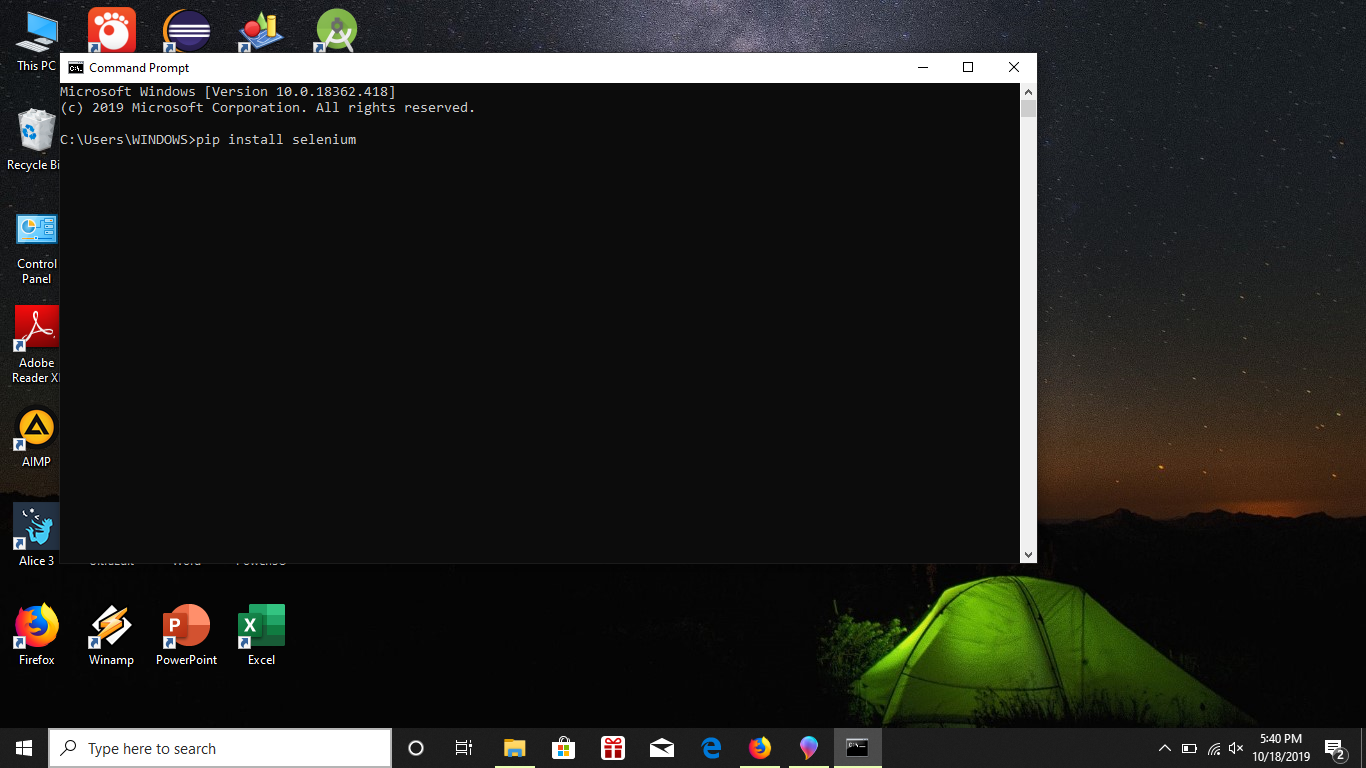
\includegraphics[width=8cm]{image/pipinstallsel.png}}
    \item Download driver, disini saya menggunakan chrome driver. Download driver sesuai browser anda
        \begin{figure}[h]
            \centerline{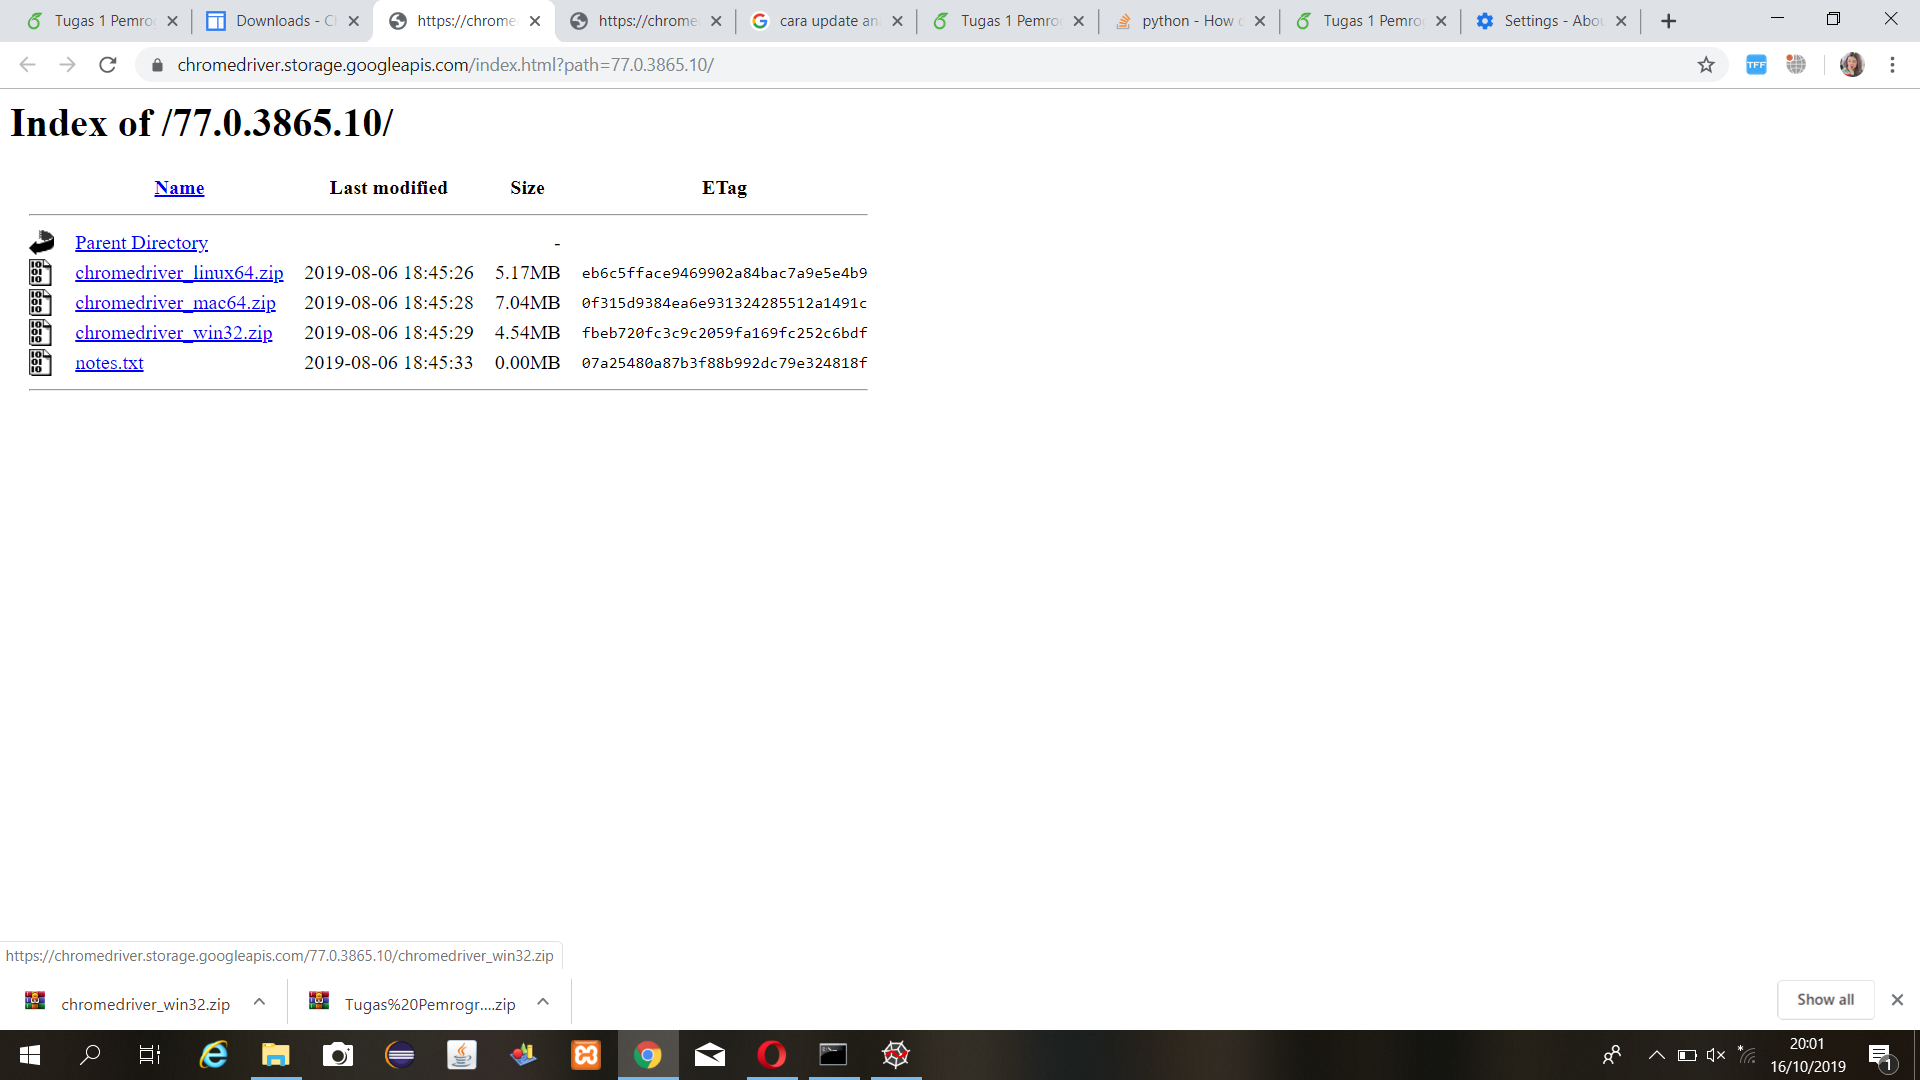
\includegraphics[width=8cm]{image/chromedriver.png}}
        \end{figure}
    \item Lalu ketikkan script berikut di Spyder
        \begin{figure}[h]
            \centerline{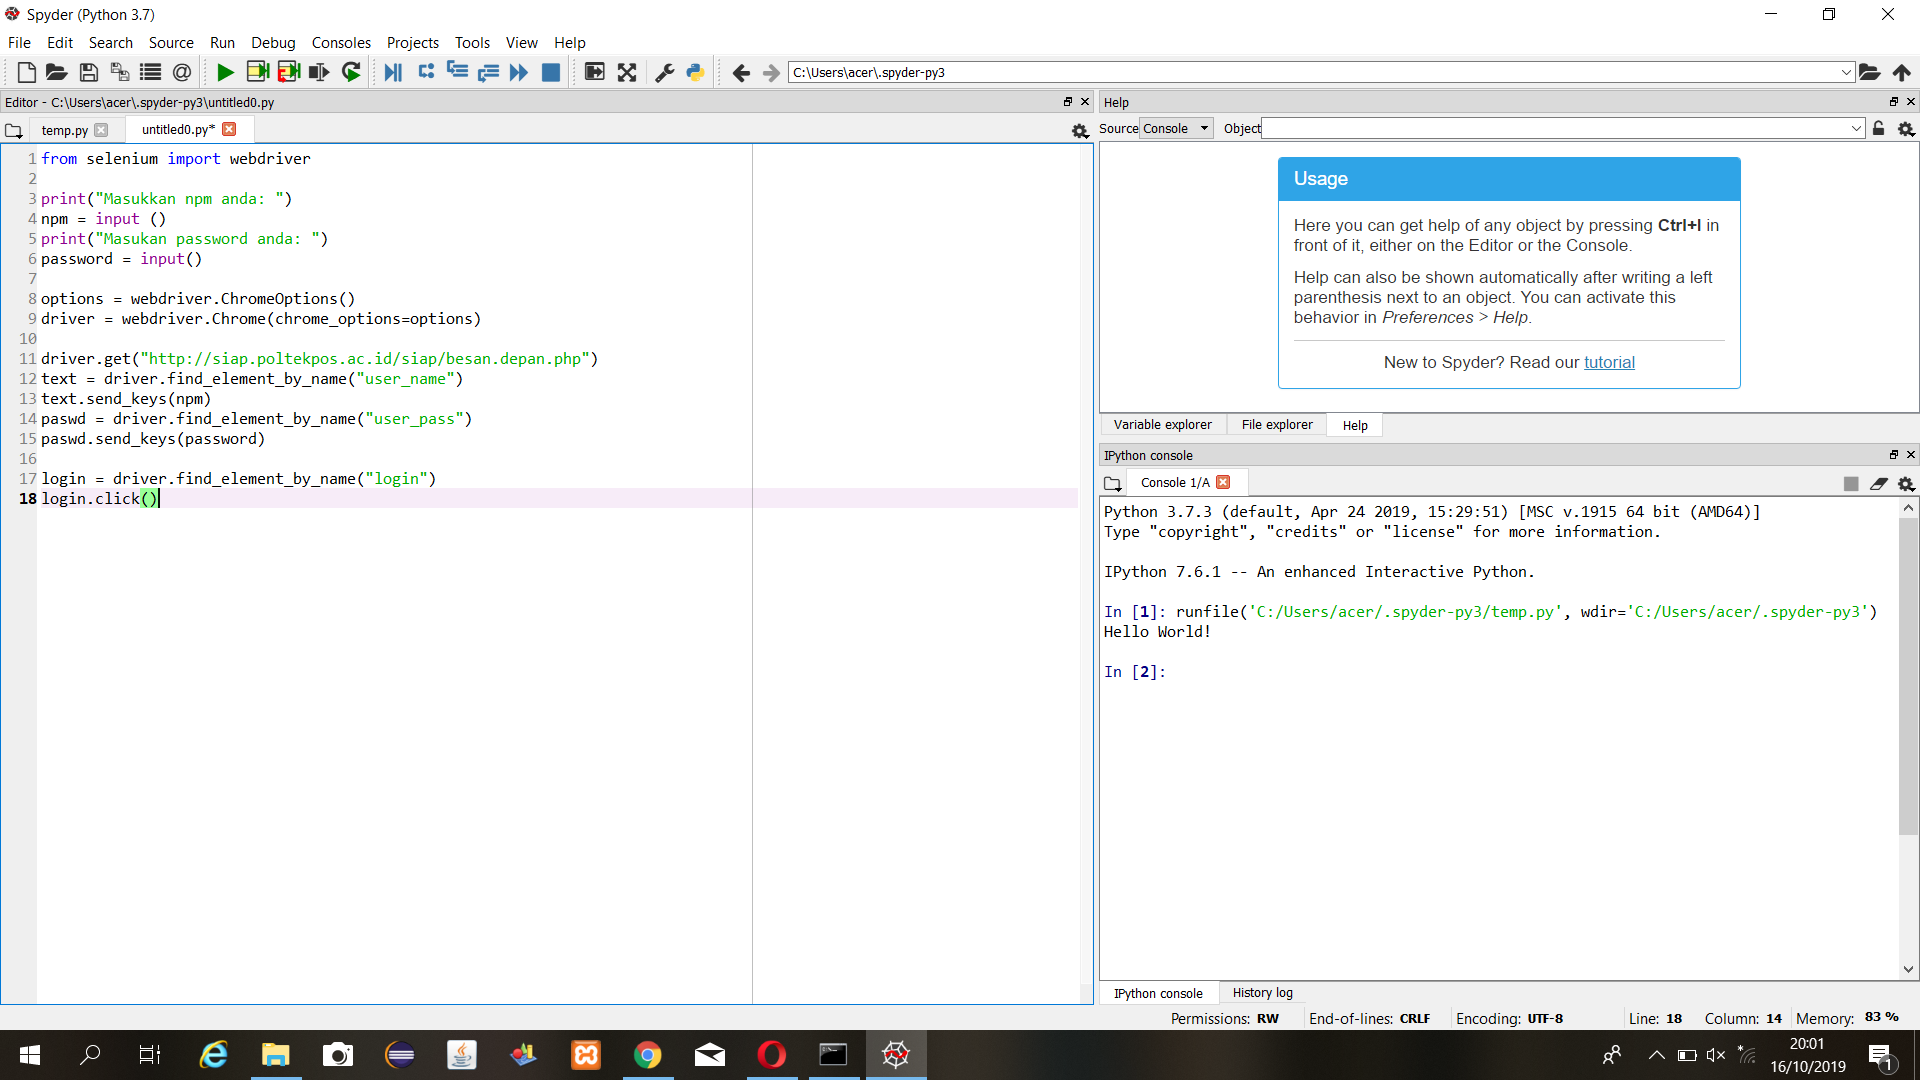
\includegraphics[width=8cm]{image/scriptsele.png}}
        \end{figure}
    \item Lalu run, setelah itu akan login otomatis ke browser yang anda tuju
\end{enumerate}
\newpage
\subsection{Cara Menggunakan Variabel Explorer pada Spyder}
\begin{enumerate}
    \item Buka aplikasi Spyder pada PC/laptop anda
    \item Pada program anda, tambahkan variabel a yang bertipe integer nilai nya bebas, begitu pula dengan variabel b
    \item Variabel c merupakan hasil dari penjumlahan variabel a dan b, c = a+b
    \item Hasilnya akan diperlihatkan dengan jelas pada variabel explore
        \begin{figure}[h]
            \centerline{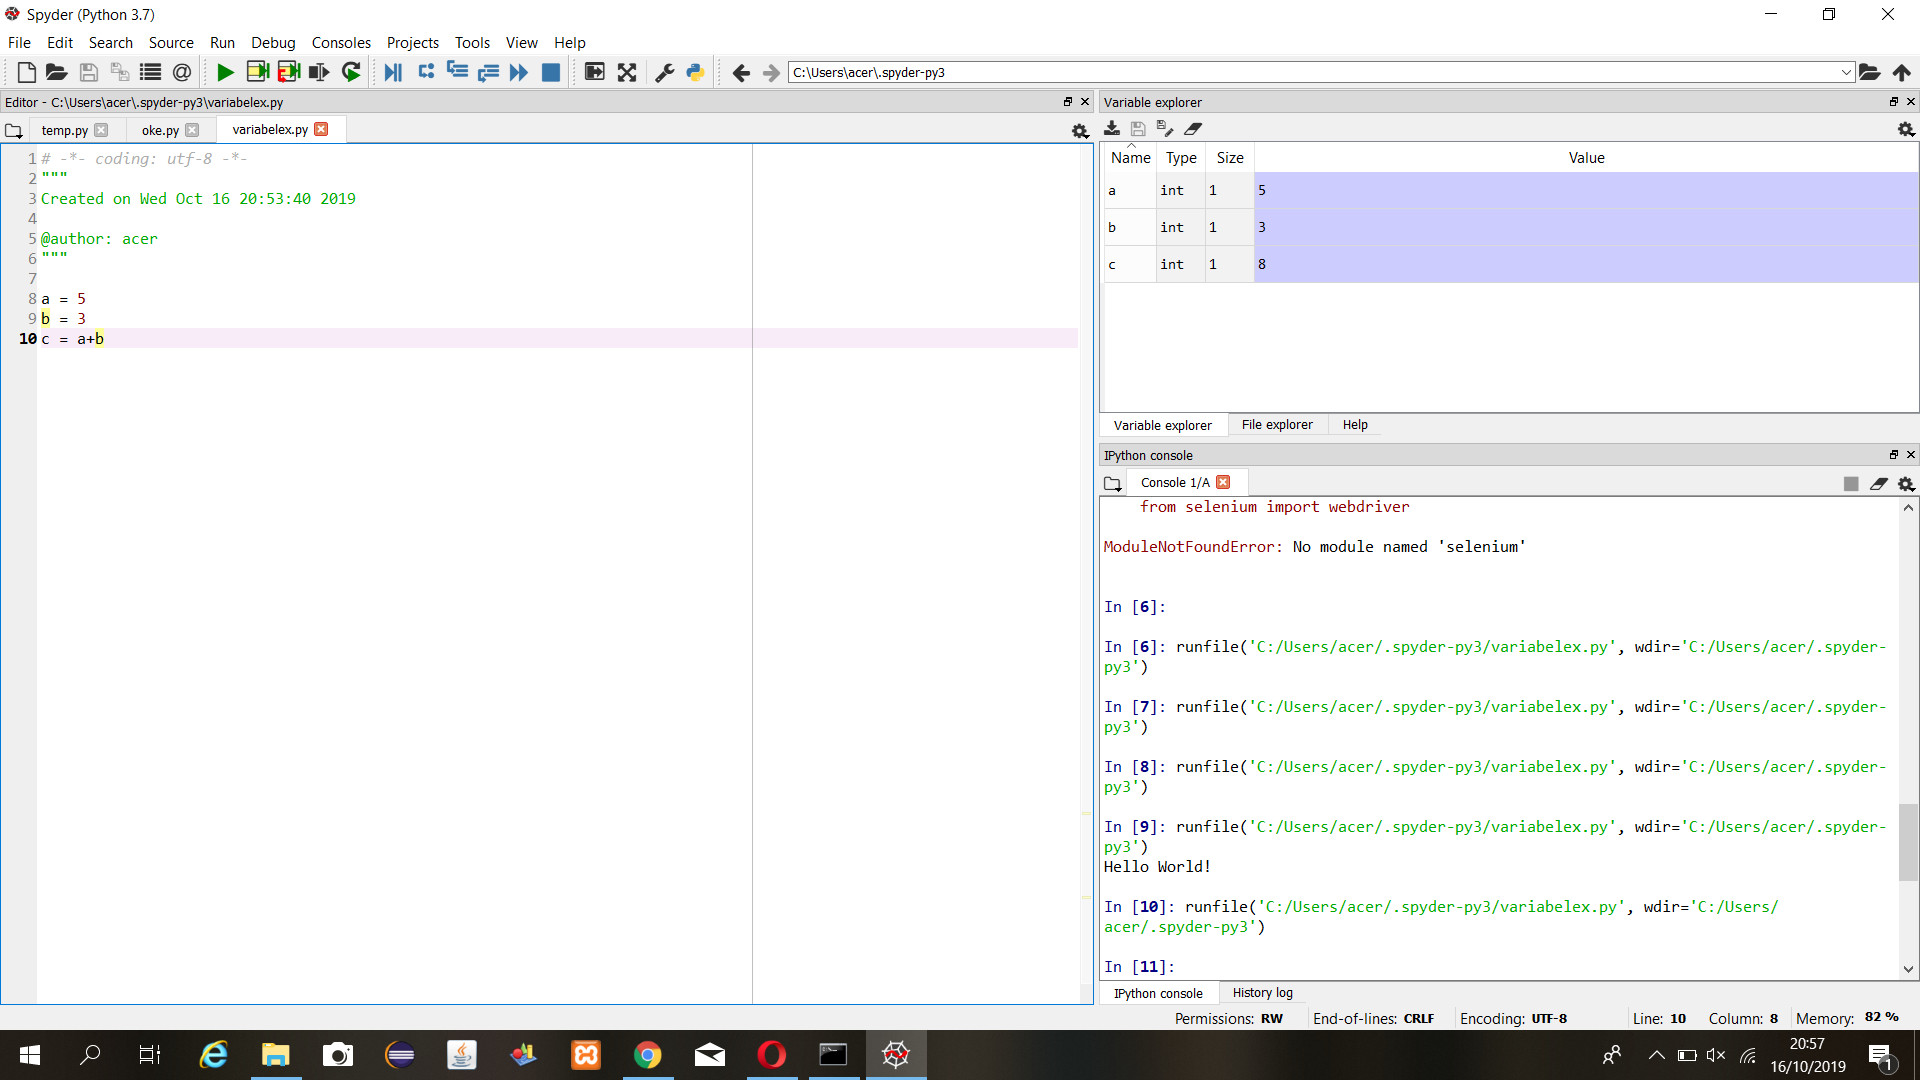
\includegraphics[width=8cm]{image/variabelex.png}}
        \end{figure}
\end{enumerate}
\newpage
\section{Identasi}
\subsection{Pengertian Identasi}
\paragraph{}
    Identasi adalah bagian awal dari paragraf yang lebih menjorok ke dalam pada setiap baris dari paragraf.
\subsection{Jenis-Jenis Error Identasi yang Ditemukan}
\begin{enumerate}
    \item Identasi If
    \item Identasi Else
    \item Identasi Elif
\end{enumerate}
\subsection{Contoh Error dan Benar}
\begin{enumerate}
    \item Contoh Error
    \paragraph{}
        \centerline{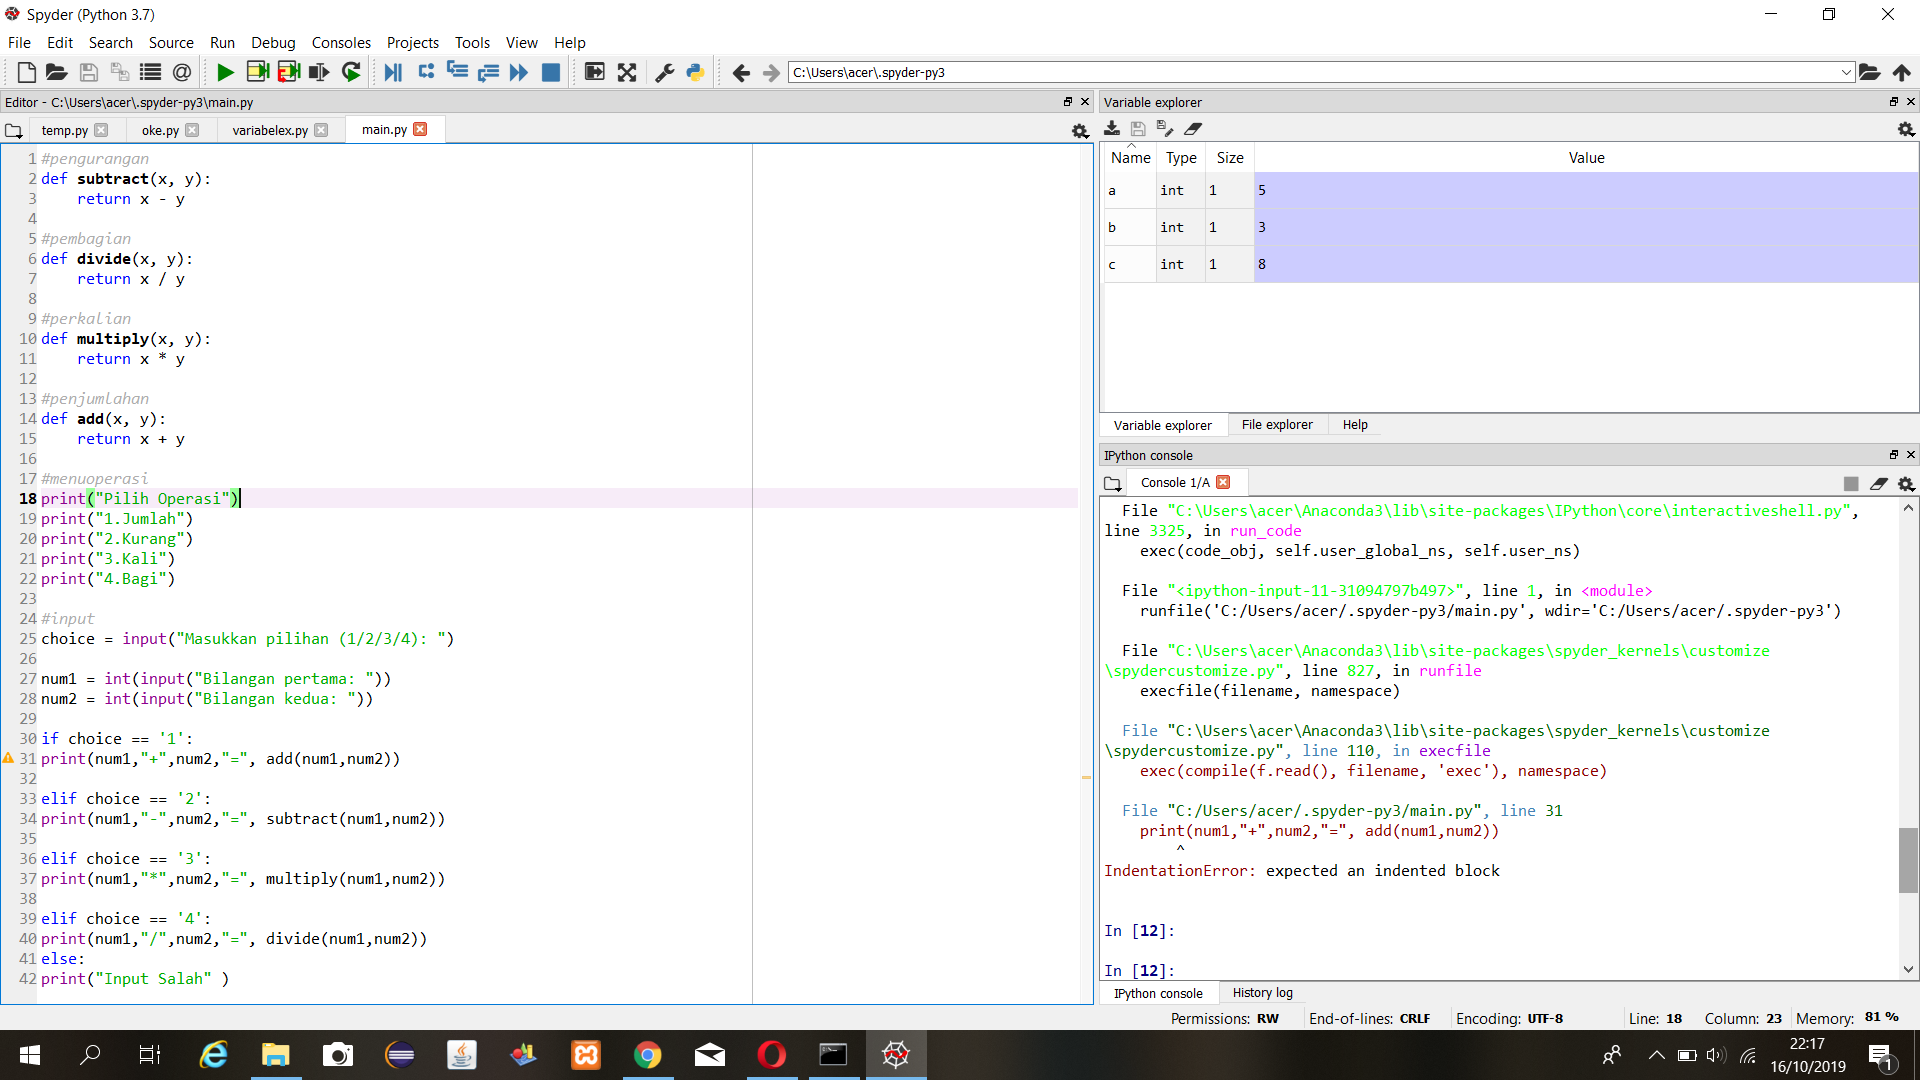
\includegraphics[width=8cm]{image/error.png}}
    \item Contoh Benar
    \begin{figure}[h]
            \centerline{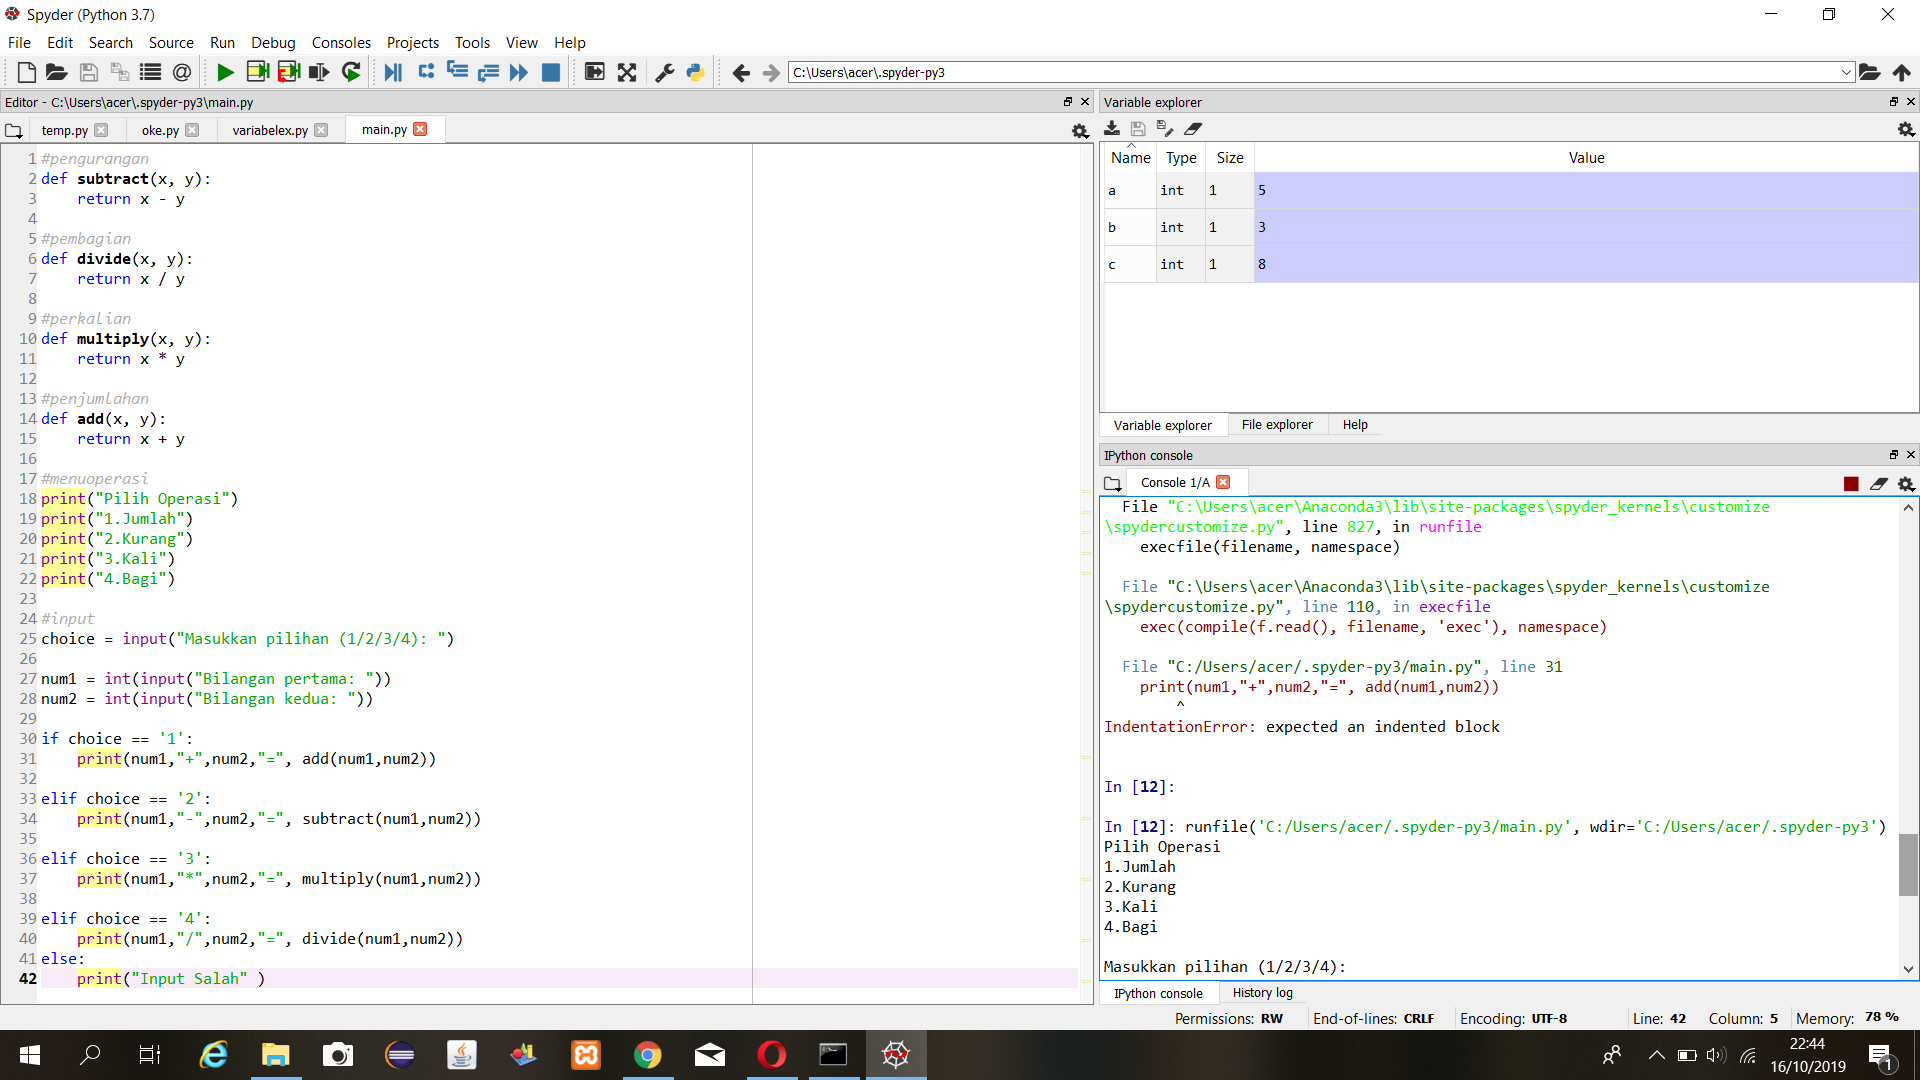
\includegraphics[width=8cm]{image/contohbenar.png}}
        \end{figure}
\end{enumerate}
\section{Link Youtube}
https://youtu.be/imlHehwNWuE
\end{document}

